% !TeX program = xelatex
% !TeX encoding = UTF-8

\documentclass[aspectratio=169, 10pt]{beamer}

% ============================================================
% IQB Beamer Theme
% ============================================================
\usepackage{../../../theme/beamerthemeiqb}
\usepackage{../../../theme/iqb-layouts}
\renewcommand{\iqbheaderimage}{../../../theme/images/header.png}
\setstretch{1.05}

\usepackage{amsmath}
\usepackage{amssymb}
\usepackage{booktabs}
% Fix protein.png path for this subdirectory
\renewcommand{\iqbsectionframe}[2]{%
  \setsection{#1}%
  \begin{frame}[plain,noframenumbering]
    \begingroup
      % Hide footer on section divider
      \setbeamertemplate{footline}{}
      % Background gradient
      \begin{tikzpicture}[remember picture,overlay]
        \fill[white] (current page.south west) rectangle (current page.north east);
        \shade[left color=white, right color=iqblightgray!30]
              (current page.south west) rectangle (current page.north east);
      \end{tikzpicture}
      % Left vertical bar
      \begin{tikzpicture}[remember picture,overlay]
        \draw[line width=8pt, color=iqbblue]
             (current page.north west) -- (current page.south west);
      \end{tikzpicture}
      % Decorative protein (FIXED PATH)
      \begin{tikzpicture}[remember picture,overlay]
        \node[anchor=south east, inner sep=0pt, opacity=0.12]
             at ($(current page.south east) + (-1cm, 1cm)$) {
          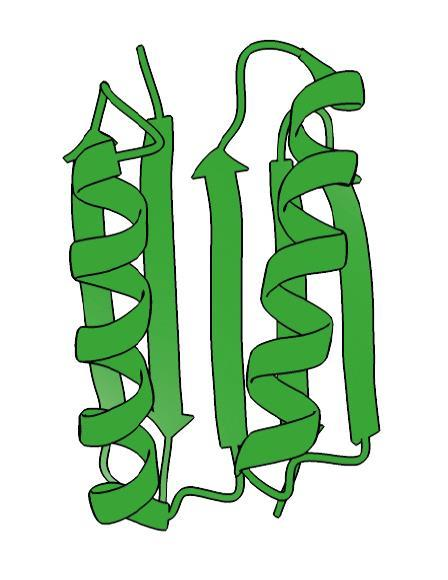
\includegraphics[height=5cm,keepaspectratio]{../../../theme/images/protein.png}
        };
      \end{tikzpicture}
      % Title
      \vspace*{0.5cm}
      \begin{center}
        {\Huge\color{iqbblue}\textbf{#2}}\\[0.3cm]
        {\Large\color{iqbgray}#1}
      \end{center}
      \vspace*{0.3cm}
    \endgroup
  \end{frame}
}

% 缩小子项缩进（本课程讲义使用更紧凑的层级）
\renewcommand{\subitem}[1]{%
  \par\vspace{2pt}%
  \noindent\hspace{0.8em}\textcolor{iqbblue}{$\circ$}\ #1%
}


% ============================================================
% Meta Information
% ============================================================
% 设置教材信息
\iqbtextbook{Quantum Chemistry}{Levine}{7th Edition}{Pearson}

% 课程讲义元数据
\lecturetitle{第三章：算符理论}
\lectureengtitle{Chapter 3: Operators, Algebra, and Eigenvalue Problems}

\author{东山月光下QM小组}
\date{\today}

% ============================================================
% Document Start
% ============================================================
\begin{document}

% ============================================================
% Title Frame
% ============================================================
\iqbcoverframe

% ============================================================
% Overview
% ============================================================
\begin{frame}{本章概览：算符理论的完整框架}
  \begin{iqbitemize}
    \item \textbf{算符基础}（Operator Basics）：定义、线性算符、常见算符实例
    \item \textbf{算符代数}（Operator Algebra）：加法、乘法、幂运算、算符函数
    \item \textbf{对易关系}（Commutation Relations）：对易子及其物理意义
    \item \textbf{本征值问题}（Eigenvalue Problems）：本征方程、可观测量、完备性
  \end{iqbitemize}

  \iqbbigsep

  \iqbgreenbox{核心思想}{算符是量子力学的语言，将物理量转化为数学对象}
\end{frame}

% ============================================================
% Section 3.1: Operators
% ============================================================
\iqbsectionframe{Section 3.1}{算符基础 (Operators)}

\begin{frame}{什么是算符？从薛定谔方程说起}
  
  \iqblayouttwo{
    \iqbsectiontitle{从薛定谔方程引入算符}
    \begin{iqbitemize}
      \item \textbf{定态薛定谔方程}（time-independent Schrödinger equation）可以写成算符形式
      \[
        \left[-\dfrac{\hbar^2}{2m}\dfrac{\mathrm{d}^2}{\mathrm{d}x^2} + V(x)\right]\psi(x) = E\psi(x)
      \]
      \item 方括号内的整体是一个\textbf{算符}（operator），称为\textbf{哈密顿算符}（Hamiltonian operator）$\hat{H}$
      \item 算符作用在\textbf{波函数}（wave function）$\psi(x)$上，产生同样的波函数乘以能量$E$
      \item 这启示我们：算符是量子力学描述物理量的数学语言
    \end{iqbitemize}

    \iqbtinysep

    \iqbsectiontitle{算符的直观理解}
    \begin{iqbitemize}
      \item 算符是一个\textbf{操作规则}或\textbf{变换指令}
      \item 它接受一个函数作为输入，输出另一个函数
      \item 就像机器：输入原料（函数）→ 加工处理 → 输出产品（新函数）
      \item 用帽子符号$\hat{\ }$标记算符，以区别于普通数字
    \end{iqbitemize}
  }{
    \iqbsectiontitle{具体例子}
    \begin{iqbitemize}
      \item \textbf{微分算符}（differential operator）$\hat{D} = \dfrac{\mathrm{d}}{\mathrm{d}x}$
      \[
        \hat{D}(x^2 + 3e^{2x}) = 2x + 6e^{2x}
      \]
      对原函数求导，得到新函数

      \item \textbf{乘法算符}$\hat{3}$（乘以3）
      \[
        \hat{3}(x + e^{x}) = 3x + 3e^{x}
      \]
      将原函数整体乘以3

      \item \textbf{三角算符}$\hat{T}$：
      \[
        \hat{T}f(x) = \tan[f(x)]
      \]
      对函数取正切
    \end{iqbitemize}

    \iqborangebox{核心概念}{算符不是数值而是对函数进行变换的操作或规则}
  }
\end{frame}

\begin{frame}{算符运算遵循严格的代数规则}
  
  \iqblayouttwo{
    \iqbsectiontitle{算符的加法与减法}
    \begin{iqbitemize}
      \item \textbf{定义}：两个算符的和（差）逐个作用后相加（减）
      \[
        (\hat{A} \pm \hat{B})f(x) = \hat{A}f(x) \pm \hat{B}f(x)
      \]

      \item \textbf{例子}：设$\hat{D} = \dfrac{\mathrm{d}}{\mathrm{d}x}$，$\hat{3}$为乘以3
      \[
        (\hat{D} + \hat{3})(x^3 - 5x) = \hat{D}(x^3 - 5x) + \hat{3}(x^3 - 5x)
      \]
      \[
        = (3x^2 - 5) + (3x^3 - 15x) = 3x^3 + 3x^2 - 15x - 5
      \]

      \item 算符加法满足\textbf{交换律}：$\hat{A} + \hat{B} = \hat{B} + \hat{A}$

      \item 算符加法满足\textbf{结合律}：$(\hat{A} + \hat{B}) + \hat{C} = \hat{A} + (\hat{B} + \hat{C})$
    \end{iqbitemize}
  }{
    \iqbsectiontitle{算符的乘积}
    \begin{iqbitemize}
      \item \textbf{关键规则}：从右向左依次作用
      \[
        \hat{A}\hat{B}f(x) = \hat{A}[\hat{B}f(x)]
      \]
      先作用右边的$\hat{B}$，再对结果作用左边的$\hat{A}$

      \item \textbf{例子}：$\hat{3}\hat{D}f(x)$
      \[
        \hat{3}\hat{D}f(x) = \hat{3}[\hat{D}f(x)] = \hat{3}[f'(x)] = 3f'(x)
      \]
      先求导，再乘以3

      \item \textbf{重要}：算符乘法\textbf{一般不满足交换律}
      \[
        \hat{A}\hat{B} \neq \hat{B}\hat{A}
      \]
      顺序不同，结果可能不同

      \item 这是量子力学与经典力学的\textbf{根本区别}
    \end{iqbitemize}

    \iqbgreenbox{核心}{算符乘积的顺序至关重要，这是\textbf{对易关系}（commutation relation）的起源}
  }
\end{frame}

\begin{frame}{算符等式与代数规则}
  \iqblayouttwo{
    \iqbsectiontitle{算符相等的严格定义}
    \begin{iqbitemize}
    \item \textbf{数学定义}（operator equality）
    \end{iqbitemize}
      \[
        \hat{A} = \hat{B} \quad \text{当且仅当} \quad \hat{A}f = \hat{B}f \quad \text{对所有函数}f
      \]
    \begin{iqbitemize}
    \item 两算符相等意味着对任意函数的作用结果相同
    \item \textbf{常见错误}：不能仅从一次作用就判断算符相等
    \end{iqbitemize}
      \[
        \frac{d}{dx}e^{2x} = 2e^{2x} \quad \text{但} \quad \frac{d}{dx} \neq 2
      \]
    \begin{iqbitemize}
    \item 因为等式不对所有函数成立（例如对$x^2$不成立）
    \end{iqbitemize}
  }{
    \iqbsectiontitle{算符代数的基本规则}
    \begin{iqbitemize}
    \item \textbf{结合律}（associative）：
    \[
      (\hat{A}\hat{B})\hat{C} = \hat{A}(\hat{B}\hat{C})
    \]
    \item \textbf{分配律}（distributive）：
    \[
      \hat{A}(\hat{B} + \hat{C}) = \hat{A}\hat{B} + \hat{A}\hat{C}
    \]
    \item \textbf{交换律不成立}（non-commutative）：
    \[
      \hat{A}\hat{B} \neq \hat{B}\hat{A} \quad \text{（一般情况）}
    \]
    \item 这是算符代数与普通代数的\textbf{根本区别}
    \end{iqbitemize}
    \iqbtinysep

    \iqbgreenbox{关键洞察}{算符乘法顺序影响结果，体现量子力学的本质特征}
  }
\end{frame}

\begin{frame}{算符等式的推导：对易关系的起源}
  \iqblayouttwo{
    \iqbsectiontitle{推导目标}
    \begin{iqbitemize}
    \item 证明微分算符与乘法算符的重要关系：
    \end{iqbitemize}
      \[
        \boxed{\hat{D}\hat{x} = \hat{1} + \hat{x}\hat{D}}
      \]
    \begin{iqbitemize}
    \item \textbf{方法}：利用算符相等定义，证明两边对任意函数$f(x)$作用结果相同
    \end{iqbitemize}
    \iqbtinysep

    \iqbsectiontitle{左边作用：$\hat{D}\hat{x}f(x)$}
    \begin{iqbitemize}
    \item 计算：$\dfrac{\mathrm{d}}{\mathrm{d}x}[xf(x)]$
    \item 使用乘积求导法则：$(uv)' = u'v + uv'$
    \end{iqbitemize}
      \[
        \dfrac{\mathrm{d}}{\mathrm{d}x}[xf(x)] = 1 \cdot f(x) + x \cdot f'(x) = f(x) + x\dfrac{\mathrm{d}f}{\mathrm{d}x}
      \]
  }{
    \iqbsectiontitle{右边作用：$(\hat{1} + \hat{x}\hat{D})f(x)$}
    \begin{iqbitemize}
    \item 计算：$\hat{1}f(x) + \hat{x}\hat{D}f(x)$
    \end{iqbitemize}
      \[
        f(x) + x\dfrac{\mathrm{d}f}{\mathrm{d}x}
      \]
    \begin{iqbitemize}
    \item 与左边结果\textbf{完全相同}
    \end{iqbitemize}
    \iqbsmallsep

    \iqbsectiontitle{关键结论}
    \begin{iqbitemize}
    \item $\hat{D}\hat{x} - \hat{x}\hat{D} = \hat{1}$
    \item 定义对易子：$[\hat{D}, \hat{x}] = \hat{D}\hat{x} - \hat{x}\hat{D} = \hat{1}$
    \item 这是\textbf{海森堡不确定性原理}的数学基础
    \end{iqbitemize}
    \iqbtinysep

    \iqbgreenbox{物理意义}{位置算符与动量算符不可对易，导致位置和动量不能同时精确测量}
  }
\end{frame}

\begin{frame}{算符的线性：为什么如此重要？（1/2）}
  
  
    \iqbsectiontitle{线性算符的直观理解}
    \begin{iqbitemize}
      \item \textbf{叠加性的物理意义}
      \begin{itemize}
        \setlength{\itemsep}{0.05cm}
        \item 如果系统可以处于状态$\psi_1$或$\psi_2$
        \item 那么也可以处于它们的\textbf{线性组合}（linear combination）$c_1\psi_1 + c_2\psi_2$
        \item 这是\textbf{量子叠加原理}（quantum superposition principle）的数学表达
      \end{itemize}

      \item \textbf{齐次性的物理意义}
      \begin{itemize}
        \setlength{\itemsep}{0.05cm}
        \item 将波函数整体放大或缩小$c$倍
        \item 不改变系统的物理状态
        \item 因为概率密度$|\psi|^2$会相应缩放，但归一化条件保持比例
      \end{itemize}

      \item \textbf{为什么量子力学算符必须是线性的？}
      \begin{itemize}
        \setlength{\itemsep}{0.05cm}
        \item 实验观察：量子态满足叠加原理
        \item 数学要求：薛定谔方程是\textbf{线性微分方程}（linear differential equation）
        \item 物理后果：保证概率诠释的一致性
      \end{itemize}
    \end{iqbitemize}
  
\end{frame}

\begin{frame}{算符的线性：为什么如此重要？（2/2）}
  \iqbfontsizemode{small}
  
    \iqbsectiontitle{线性的数学验证}
    \begin{iqbitemize}
      \item \textbf{验证拉普拉斯算符的线性}
      \[
        \nabla^2 = \dfrac{\partial^2}{\partial x^2} + \dfrac{\partial^2}{\partial y^2} + \dfrac{\partial^2}{\partial z^2}
      \]

      \item \textbf{叠加性验证}
      \begin{align*}
        \nabla^2(f+g) &= \dfrac{\partial^2(f+g)}{\partial x^2} + \cdots \\
                  &= \dfrac{\partial^2 f}{\partial x^2} + \dfrac{\partial^2 g}{\partial x^2} + \cdots \\
                  &= \nabla^2 f + \nabla^2 g
      \end{align*}

      \item \textbf{齐次性验证}
      \begin{align*}
        \nabla^2(cf) &= \dfrac{\partial^2(cf)}{\partial x^2} + \cdots \\
                 &= c\dfrac{\partial^2 f}{\partial x^2} + \cdots \\
                 &= c\nabla^2 f
      \end{align*}

      \item \textbf{非线性的反例}
      \[
        \sqrt{\hat{\ }}f(x) = \sqrt{f(x)}
      \]
      显然$\sqrt{f+g} \neq \sqrt{f} + \sqrt{g}$，不满足线性
    \end{iqbitemize}
  

\end{frame}

\begin{frame}{线性算符（1/2）}
  
  
    \iqbsectiontitle{线性算符的定义}
    \begin{iqbitemize}
    \item 算符$\hat{A}$是线性的，当且仅当满足两个条件
    \end{iqbitemize}
    \iqbsmallsep

    \iqbsectiontitle{条件1：叠加性（additivity）}
    \begin{iqbitemize}
    \item 数学表达：
    \end{iqbitemize}
      \[
        \hat{A}[f(x) + g(x)] = \hat{A}f(x) + \hat{A}g(x)
      \]
    \begin{iqbitemize}
    \item 物理意义：两个函数之和的算符作用等于各函数算符作用之和
    \item 这允许我们将复杂状态分解为简单状态的叠加
    \end{iqbitemize}
    \iqbsmallsep

    \iqbsectiontitle{条件2：齐次性（homogeneity）}
    \begin{iqbitemize}
    \item 数学表达：
    \end{iqbitemize}
      \[
        \hat{A}[c \cdot f(x)] = c \cdot \hat{A}f(x)
      \]
    \begin{iqbitemize}
    \item 物理意义：常数倍函数的算符作用等于常数倍的算符作用
    \item 确保算符作用保持波函数的归一化性质
    \end{iqbitemize}
  
\end{frame}

\begin{frame}{线性算符（2/2 上）}
  
  
    \iqbsectiontitle{为什么量子力学需要线性算符？}
    \begin{iqbitemize}
    \item \textbf{叠加原理的数学基础}
    \subitem{量子系统可以处于多个状态的叠加}
    \subitem{例如：$\Psi = c_1\psi_1 + c_2\psi_2$}
    \item \textbf{态的线性演化}
    \subitem{薛定谔方程是线性的}
    \subitem{初始态的线性叠加演化为末态的线性叠加}
    \item \textbf{测量理论的要求}
    \subitem{本征函数构成完备集}
    \subitem{任意态可展开为本征态的叠加}
    \end{iqbitemize}
    \iqbsmallsep

    \end{frame}

\begin{frame}{线性算符（2/2 下）}
  
  
    \iqbsectiontitle{常见线性算符实例}
    \begin{iqbitemize}
    \item 微分算符：$\hat{D} = \dfrac{\mathrm{d}}{\mathrm{d}x}$
    \item Laplace算符：$\nabla^2 = \dfrac{\partial^2}{\partial x^2} + \dfrac{\partial^2}{\partial y^2} + \dfrac{\partial^2}{\partial z^2}$
    \item 哈密顿算符：$\hat{H} = -\dfrac{\hbar^2}{2m}\nabla^2 + V$
    \item 乘法算符：$\hat{x}$、$\hat{p}$、$\hat{V}(x)$
    \end{iqbitemize}
    \iqbsmallsep

    \iqborangebox{关键洞察}{线性确保量子态的演化保持幺正性，概率守恒}
  

\end{frame}

\begin{frame}{算符代数：乘法顺序至关重要}
  
  \iqblayouttwo{
    \iqbsectiontitle{算符的加减}
    \begin{iqbitemize}
      \item 两个算符之和定义为：
      \[
        (\hat{A} + \hat{B})f(x) = \hat{A}f(x) + \hat{B}f(x)
      \]
      \item 两个算符之差定义为：
      \[
        (\hat{A} - \hat{B})f(x) = \hat{A}f(x) - \hat{B}f(x)
      \]
      \item 算符加减后仍是算符
      \item 加法满足交换律：$\hat{A} + \hat{B} = \hat{B} + \hat{A}$
    \end{iqbitemize}
  }{
    \iqbsectiontitle{算符的乘积}
    \begin{iqbitemize}
      \item 算符乘积定义为连续作用：
      \[
        \hat{A}\hat{B}f(x) = \hat{A}[\hat{B}f(x)]
      \]
      \item 先作用右边的算符$\hat{B}$，再作用左边的算符$\hat{A}$

      \iqbtinysep

      \item \textbf{重要}：算符乘法一般\textbf{不满足交换律}
      \[
        \hat{A}\hat{B} \neq \hat{B}\hat{A}
      \]

      \iqbtinysep

      \item 这是量子力学与经典力学的重要区别
    \end{iqbitemize}
  }
\end{frame}

\begin{frame}{验证算符线性：叠加原理的数学证明（1/2）}
  
    \iqbsectiontitle{问题设定}
    \begin{iqbitemize}
    \item 设$\hat{A} = \dfrac{\mathrm{d}}{\mathrm{d}x}$（微分算符），$\hat{B} = x$（乘法算符）
    \item 计算$\hat{A}\hat{B}$和$\hat{B}\hat{A}$并比较
    \item 验证它们是否相等（即是否对易）
    \end{iqbitemize}
    \iqbsmallsep

    \iqbsectiontitle{计算$\hat{A}\hat{B}f(x)$}
    \begin{iqbitemize}
    \item 先乘法后求导：
    \end{iqbitemize}
      \[
        \hat{A}\hat{B}f(x) = \dfrac{\mathrm{d}}{\mathrm{d}x}[x f(x)]
      \]
    \begin{iqbitemize}
    \item 使用乘积法则：$(uv)' = u'v + uv'$
    \end{iqbitemize}
      \[
        = f(x) + x f'(x) = (1 + x\dfrac{\mathrm{d}}{\mathrm{d}x})f(x)
      \]
  
\end{frame}

\begin{frame}{验证算符线性：叠加原理的数学证明（2/2 上）}
  
    \iqbsectiontitle{计算$\hat{B}\hat{A}f(x)$}
    \begin{iqbitemize}
    \item 先求导后乘法：
    \end{iqbitemize}
      \[
        \hat{B}\hat{A}f(x) = x \cdot \dfrac{\mathrm{d}}{\mathrm{d}x}f(x)
      \]
    \begin{iqbitemize}
    \item 直接对$f(x)$求导再乘$x$：
    \end{iqbitemize}
      \[
        = x f'(x) = (x\dfrac{\mathrm{d}}{\mathrm{d}x})f(x)
      \]
    \iqbsmallsep

    \end{frame}

\begin{frame}{验证算符线性：叠加原理的数学证明（2/2 下）}
  
    \iqbsectiontitle{对比与结论}
    \begin{iqbitemize}
    \item $\hat{A}\hat{B} = 1 + x\dfrac{\mathrm{d}}{\mathrm{d}x}$
    \item $\hat{B}\hat{A} = x\dfrac{\mathrm{d}}{\mathrm{d}x}$
    \item \textbf{相差恒等算符}：
    \end{iqbitemize}
      \[
        \hat{A}\hat{B} - \hat{B}\hat{A} = \hat{1} \quad \Rightarrow \quad [\hat{A}, \hat{B}] = \hat{1}
      \]
    \begin{iqbitemize}
    \item 这就是著名的对易关系！
    \end{iqbitemize}
    \iqbsmallsep

    \iqbgreenbox{物理意义}{算符顺序改变结果，是量子力学区别于经典力学的本质特征}
  

\end{frame}

% ============================================================
% Example 3.1: Operator Algebra
% ============================================================
\begin{frame}{例题3.1：验证算符代数恒等式}
  \iqbfontsizemode{small}
  \iqbsectiontitle{验证$(\hat{A} + \hat{B})^2 \neq \hat{A}^2 + 2\hat{A}\hat{B} + \hat{B}^2$}

  \textbf{问题}：设$\hat{A} = \dfrac{\mathrm{d}}{\mathrm{d}x}$，$\hat{B} = x$，验证算符平方展开

  \iqbsep

  \begin{iqbitemize}
    \item \textbf{经典代数}：$(a+b)^2 = a^2 + 2ab + b^2$

    \item \textbf{算符代数}：一般\textcolor{red}{不成立}！
    \[
      (\hat{A} + \hat{B})^2 = (\hat{A} + \hat{B})(\hat{A} + \hat{B}) = \hat{A}^2 + \hat{A}\hat{B} + \hat{B}\hat{A} + \hat{B}^2
    \]

    \item \textbf{验证}：左边$(\hat{D} + \hat{x})^2 = (\hat{D} + \hat{x})(\hat{D} + \hat{x})$
    \begin{align*}
      &= \hat{D}^2 + \hat{D}\hat{x} + \hat{x}\hat{D} + \hat{x}^2 \\
      &= \hat{D}^2 + (\hat{1} + \hat{x}\hat{D}) + \hat{x}\hat{D} + \hat{x}^2 \\
      &= \hat{D}^2 + \hat{1} + 2\hat{x}\hat{D} + \hat{x}^2
    \end{align*}

    \item \textbf{右边}：$\hat{A}^2 + 2\hat{A}\hat{B} + \hat{B}^2 = \hat{D}^2 + 2\hat{D}\hat{x} + \hat{x}^2$

    \item \textbf{比较}：
    \begin{itemize}
      \setlength{\itemsep}{0.05cm}
      \item 左边展开：$\hat{D}^2 + \hat{1} + 2\hat{x}\hat{D} + \hat{x}^2$
      \item 右边展开：$\hat{D}^2 + 2\hat{D}\hat{x} + \hat{x}^2$
      \item 差值：$\hat{1} + 2\hat{x}\hat{D} - 2\hat{D}\hat{x}$
      \item 由于$2\hat{x}\hat{D} \neq 2\hat{D}\hat{x}$，两边不相等
    \end{itemize}
  \end{iqbitemize}

  \iqbgreenbox{结论}{算符代数必须严格按照定义展开，不能套用经典代数公式}
\end{frame}

\begin{frame}{例题3.2：算符多项式的计算}
  \iqbfontsizemode{small}
  \iqbsectiontitle{计算$(\hat{A}+\hat{B})^3$的展开式}

  \textbf{问题}：展开算符多项式$(\hat{A}+\hat{B})^3$并说明需要注意的问题

  \iqbsep

  \begin{iqbitemize}
    \item \textbf{错误的展开}（套用经典代数）：
    \[
      (\hat{A}+\hat{B})^3 \neq \hat{A}^3 + 3\hat{A}^2\hat{B} + 3\hat{A}\hat{B}^2 + \hat{B}^3
    \]

    \item \textbf{正确的展开}（保持算符顺序）：
    \begin{align*}
      (\hat{A}+\hat{B})^3 &= (\hat{A}+\hat{B})(\hat{A}+\hat{B})(\hat{A}+\hat{B}) \\
      &= (\hat{A}+\hat{B})(\hat{A}^2 + \hat{A}\hat{B} + \hat{B}\hat{A} + \hat{B}^2) \\
      &= \hat{A}^3 + \hat{A}^2\hat{B} + \hat{A}\hat{B}\hat{A} + \hat{A}\hat{B}^2 \\
      &\quad + \hat{B}\hat{A}^2 + \hat{B}\hat{A}\hat{B} + \hat{B}^2\hat{A} + \hat{B}^3
    \end{align*}

    \item \textbf{关键区别}：
    \begin{itemize}
      \setlength{\itemsep}{0.05cm}
      \item 经典代数：$a^2b = ab^2 = ab^2$（乘法可交换）
      \item 算符代数：$\hat{A}^2\hat{B} \neq \hat{A}\hat{B}\hat{A} \neq \hat{B}\hat{A}^2$（顺序重要）
      \item 所有\textbf{8项}都不能合并，每一项都代表不同的作用顺序
    \end{itemize}

    \item \textbf{特例}：如果$\hat{A}$和$\hat{B}$对易（即$[\hat{A},\hat{B}]=0$），则经典公式成立
    \[
      [\hat{A},\hat{B}]=0 \Rightarrow \hat{A}\hat{B} = \hat{B}\hat{A}
    \]
    此时8项可以合并为4项
  \end{iqbitemize}

  \iqbgreenbox{关键}{算符乘法必须保持顺序，只有对易的算符才能交换}
\end{frame}

% ============================================================
% Section 3.2: Operator Algebra
% ============================================================
\iqbsectionframe{Section 3.2}{算符代数 (Operator Algebra)}

\begin{frame}{算符的幂运算}
  
  \iqblayouttwo{
    \iqbsectiontitle{定义与性质}
    \begin{iqbitemize}
      \item 算符的$n$次幂定义为连续作用$n$次
      \[
        \hat{A}^n f(x) = \underbrace{\hat{A}\hat{A}\cdots\hat{A}}_{n\text{次}}f(x)
      \]

      \item 例如：$(\dfrac{\mathrm{d}}{\mathrm{d}x})^2 f(x) = \dfrac{\mathrm{d}^2f}{\mathrm{d}x^2}$

      \item 指数律成立：$\hat{A}^m \hat{A}^n = \hat{A}^{m+n}$

      \item 算符函数可用幂级数定义
      \[
        e^{\hat{A}} = \hat{1} + \hat{A} + \dfrac{\hat{A}^2}{2!} + \dfrac{\hat{A}^3}{3!} + \cdots
      \]
    \end{iqbitemize}
  }{
    \iqbsectiontitle{实际应用}
    \begin{iqbitemize}
      \item \textbf{动能算符}：
      \[
        \hat{T} = -\dfrac{\hbar^2}{2m}\dfrac{\mathrm{d}^2}{\mathrm{d}x^2}
      \]
      涉及二阶导数算符

      \item \textbf{哈密顿算符}：
      \[
        \hat{H} = \hat{T} + \hat{V}
      \]
      动能算符与势能算符之和

      \item \textbf{平移算符}：
      \[
        e^{a\dfrac{\mathrm{d}}{\mathrm{d}x}}f(x) = f(x+a)
      \]
      指数算符产生函数平移
    \end{iqbitemize}

    \iqbtinysep

    \iqborangebox{注意}{算符函数的级数展开必须收敛才有意义}
  }
\end{frame}

\begin{frame}{算符多项式与函数（1/2）}
  
  
    \iqbsectiontitle{算符多项式的定义}
    \begin{iqbitemize}
    \item 算符多项式是算符幂的线性组合
    \end{iqbitemize}
      \[
        P(\hat{A}) = c_0\hat{1} + c_1\hat{A} + c_2\hat{A}^2 + \cdots + c_n\hat{A}^n
      \]
    \begin{iqbitemize}
    \item \textbf{单算符多项式}：类似普通代数
    \[
      (\hat{A} + \hat{1})^2 = \hat{A}^2 + 2\hat{A} + \hat{1}
    \]
    \item 因为算符与自身对易：$[\hat{A}, \hat{A}] = 0$
    \end{iqbitemize}
    \iqbsmallsep

    \iqbsectiontitle{双算符多项式的复杂性}
    \begin{iqbitemize}
    \item \textbf{常见错误}：
    \[
      (\hat{A} + \hat{B})^2 \neq \hat{A}^2 + 2\hat{A}\hat{B} + \hat{B}^2
    \]
    \item 原因：$\hat{A}$与$\hat{B}$不对易
    \end{iqbitemize}
    \iqbtinysep

    \iqbsectiontitle{正确展开方式}
    \begin{iqbitemize}
    \item 保留算符顺序：
    \[
      (\hat{A} + \hat{B})^2 = \hat{A}^2 + \hat{A}\hat{B} + \hat{B}\hat{A} + \hat{B}^2
    \]
    \item 使用对易子简化：
    \[
      (\hat{A} + \hat{B})^2 = \hat{A}^2 + 2\hat{A}\hat{B} + \hat{B}^2 + [\hat{B}, \hat{A}]
    \]
    \end{iqbitemize}
  
\end{frame}

\begin{frame}{算符多项式与函数（2/2 上）}
  
  
    \iqbsectiontitle{算符函数的定义}
    \begin{iqbitemize}
    \item 通过\textbf{泰勒级数展开}（Taylor series）定义
    \[
      f(\hat{A}) = \sum_{n=0}^{\infty} \dfrac{f^{(n)}(0)}{n!}\hat{A}^n
    \]
    \item \textbf{指数算符}（exponential operator）：
    \end{iqbitemize}
      \[
        e^{\hat{A}} = \hat{1} + \hat{A} + \dfrac{1}{2!}\hat{A}^2 + \dfrac{1}{3!}\hat{A}^3 + \cdots
      \]
    \begin{iqbitemize}
    \item 物理中的重要应用：
    \subitem{时间演化算符：$e^{-i\hat{H}t/\hbar}$}
    \subitem{平移算符：$e^{a\mathrm{d}/\mathrm{d}x}$}
    \subitem{旋转算符：$e^{-i\hat{L}_z\phi/\hbar}$}
    \end{iqbitemize}
    \iqbsmallsep

    \end{frame}

\begin{frame}{算符多项式与函数（2/2 下）}
  
  
    \iqbsectiontitle{算符函数的性质}
    \begin{iqbitemize}
    \item 级数必须收敛才有意义
    \item 不同算符的函数：$f(\hat{A}, \hat{B})$展开更复杂
    \item 特殊情况：若$[\hat{A}, \hat{B}] = 0$，则$e^{\hat{A}}e^{\hat{B}} = e^{\hat{A}+\hat{B}}$
    \item 一般情况：Baker-Campbell-Hausdorff公式
    \end{iqbitemize}
    \iqbsmallsep

    \iqbgreenbox{物理意义}{算符函数描述量子态随时间、空间或角度的演化}
  

\end{frame}

% ============================================================
% Section 3.3: Commutators
% ============================================================
\iqbsectionframe{Section 3.3}{对易子 (Commutators)}

\begin{frame}{对易子的定义}
  
  \iqblayouttwo{
    \iqbsectiontitle{定义}
    \begin{iqbitemize}
      \item 两个算符$\hat{A}$和$\hat{B}$的\textbf{对易子}（commutator）定义为
      \[
        [\hat{A}, \hat{B}] = \hat{A}\hat{B} - \hat{B}\hat{A}
      \]

      \item 对易子本身也是一个算符

      \item \textbf{对易}（commute）：若$[\hat{A}, \hat{B}] = 0$，称两算符对易

      \item \textbf{不对易}（non-commute）：若$[\hat{A}, \hat{B}] \neq 0$，称两算符不对易
    \end{iqbitemize}
  }{
    \iqbsectiontitle{物理意义}
    \begin{iqbitemize}
      \item 对易子反映了物理量是否能同时精确测量

      \item \textbf{海森堡不确定性原理}的数学表述
      \[
        \Delta A \Delta B \geq \dfrac{1}{2}|\langle[\hat{A}, \hat{B}]\rangle|
      \]

      \item 对易的算符对应可同时观测的物理量

      \item 不对易的算符对应\textbf{互补的物理量}（complementary observables）
    \end{iqbitemize}

    \iqbtinysep

    \iqbgreenbox{核心}{对易关系是量子力学的核心特征}
  }
\end{frame}

\begin{frame}{对易子的基本性质（1/2）}
  
    \iqbsectiontitle{基本代数性质}
    \begin{iqbitemize}
    \item \textbf{反对称性}（antisymmetry）：
    \[
      [\hat{A}, \hat{B}] = -[\hat{B}, \hat{A}]
    \]
    \item \textbf{自对易为零}：$[\hat{A}, \hat{A}] = 0$
    \item \textbf{线性性质}（linearity）：
    \[
      [\hat{A}, c_1\hat{B} + c_2\hat{C}] = c_1[\hat{A}, \hat{B}] + c_2[\hat{A}, \hat{C}]
    \]
    \item \textbf{雅可比恒等式}（Jacobi identity）：
    \end{iqbitemize}
      \[
        [\hat{A}, [\hat{B}, \hat{C}]] + [\hat{B}, [\hat{C}, \hat{A}]] + [\hat{C}, [\hat{A}, \hat{B}]] = 0
      \]
    \begin{iqbitemize}
    \item 确保对易子运算的一致性
    \end{iqbitemize}
  
\end{frame}

\begin{frame}{对易子的基本性质（2/2）}
  \iqbfontsizemode{small}
    \iqbsectiontitle{运算规则}
    \begin{iqbitemize}
    \item \textbf{莱布尼茨规则}（Leibniz rule）：
    \end{iqbitemize}
      \[
        [\hat{A}, \hat{B}\hat{C}] = [\hat{A}, \hat{B}]\hat{C} + \hat{B}[\hat{A}, \hat{C}]
      \]
    \begin{iqbitemize}
    \item 类似微积分中的乘积求导法则
    \item 推广形式：
    \end{iqbitemize}
      \[
        [\hat{A}\hat{B}, \hat{C}] = \hat{A}[\hat{B}, \hat{C}] + [\hat{A}, \hat{C}]\hat{B}
      \]
    \begin{iqbitemize}
    \item 注意保持算符顺序！
    \end{iqbitemize}
    \iqbsmallsep

    \iqbsectiontitle{实用计算技巧}
    \begin{iqbitemize}
    \item 展开$[\hat{A}, \hat{B}]$时，先计算$\hat{A}\hat{B}$和$\hat{B}\hat{A}$
    \item 验证结果是否满足反对称性
    \item 利用已知的对易关系（如$[x, \hat{p}_x] = i\hbar$）
    \item 复杂对易子可逐步分解为简单对易子
    \end{iqbitemize}
    \iqbtinysep

    \iqbgreenbox{记忆要点}{对易子运算就像导数运算，满足线性和莱布尼茨规则}
  

\end{frame}

\begin{frame}{重要对易关系}
  
  \iqblayouttwo{
    \iqbsectiontitle{坐标与动量}
    \begin{iqbitemize}
      \item 一维情况：
      \[
        [x, \hat{p}_x] = i\hbar
      \]

      \item 三维情况：
      \[
        [x_i, \hat{p}_j] = i\hbar\delta_{ij}
      \]

      \item 这是量子力学的基本对易关系

      \item 导致海森堡不确定性原理
      \[
        \Delta x \Delta p_x \geq \dfrac{\hbar}{2}
      \]
    \end{iqbitemize}
  }{
    \iqbsectiontitle{角动量}
    \begin{iqbitemize}
      \item 角动量各分量之间不对易
      \[
        [\hat{L}_x, \hat{L}_y] = i\hbar\hat{L}_z
      \]
      \[
        [\hat{L}_y, \hat{L}_z] = i\hbar\hat{L}_x
      \]
      \[
        [\hat{L}_z, \hat{L}_x] = i\hbar\hat{L}_y
      \]

      \item 角动量平方与任意分量对易
      \[
        [\hat{L}^2, \hat{L}_i] = 0
      \]

      \item 可以同时测量$L^2$和一个分量
    \end{iqbitemize}
  }
\end{frame}

\begin{frame}{例题：计算对易子}
  \iqbfontsizemode{small}
  \iqbsectiontitle{计算$[\dfrac{\mathrm{d}}{\mathrm{d}x}, x]$}

  \textbf{方法一：直接作用在任意函数上}

  \begin{align*}
    [\dfrac{\mathrm{d}}{\mathrm{d}x}, x]f(x) &= \dfrac{\mathrm{d}}{\mathrm{d}x}(xf(x)) - x\dfrac{\mathrm{d}}{\mathrm{d}x}f(x) \\
                         &= f(x) + xf'(x) - xf'(x) \\
                         &= f(x)
  \end{align*}

  \begin{iqbitemize}
    \item 对任意$f(x)$，结果都是$f(x)$本身
    \item 因此$[\dfrac{\mathrm{d}}{\mathrm{d}x}, x] = \hat{1}$（恒等算符）
  \end{iqbitemize}

  \iqbsep

  \iqbgreenbox{推广}{}在量子力学中，$[\hat{p}_x, x] = -i\hbar$（因为$\hat{p}_x = -i\hbar\dfrac{\mathrm{d}}{\mathrm{d}x}$）
\end{frame}

% ============================================================
% Section 3.4: Eigenfunctions and Eigenvalues
% ============================================================
\iqbsectionframe{Section 3.4}{本征函数与本征值 (Eigenfunctions \& Eigenvalues)}

\begin{frame}{本征值问题：可观测量的量子化}
  
  \iqblayouttwo{
    \iqbsectiontitle{本征方程}
    \begin{iqbitemize}
      \item 算符$\hat{A}$的\textbf{本征方程}（eigenvalue equation）定义为
      \[
        \hat{A}\phi_n(x) = a_n\phi_n(x)
      \]

      \item $\phi_n(x)$：算符$\hat{A}$的\textbf{本征函数}（eigenfunction）

      \item $a_n$：对应的\textbf{本征值}（eigenvalue）

      \item 算符作用在本征函数上，结果是该函数乘以常数

      \item 这相当于求函数方程的"驻波解"
    \end{iqbitemize}
  }{
    \iqbsectiontitle{物理意义}
    \begin{iqbitemize}
      \item \textbf{本征值}是测量该物理量可能得到的结果

      \item 测量后系统处于对应\textbf{本征态}（eigenstate）

      \item \textbf{哈密顿算符}的本征值是\textbf{能级}（energy levels）
      \[
        \hat{H}\psi_n = E_n\psi_n
      \]

      \item 定态薛定谔方程就是本征值问题
    \end{iqbitemize}

    \iqbtinysep

    \iqborangebox{关键}{本征值问题连接数学与物理测量}
  }
\end{frame}

\begin{frame}{厄米算符本征函数：正交完备且实数本征值（1/2）}
  
    \iqbsectiontitle{四个基本性质}
    \begin{iqbitemize}
    \item \textbf{实数性}（real eigenvalues）
    \end{iqbitemize}
      \[
        \hat{A}\phi_n = a_n\phi_n \quad \Rightarrow \quad a_n \in \mathbb{R}
      \]
    \begin{iqbitemize}
    \item 所有本征值都是实数
    \item 测量结果必定是实数（符合物理直觉）
    \end{iqbitemize}
    \iqbtinysep

    \iqbsectiontitle{正交性}
    \begin{iqbitemize}
    \item 不同本征值的本征函数相互正交
    \end{iqbitemize}
      \[
        \int \phi_m^*(x)\phi_n(x)\mathrm{d}x = 0 \quad (m \neq n)
      \]
    \begin{iqbitemize}
    \item 类似于三维空间中不同坐标轴的正交
    \item 确保不同本征态彼此独立
    \end{iqbitemize}
  
\end{frame}

\begin{frame}{厄米算符本征函数：正交完备且实数本征值（2/2）}
  \iqbfontsizemode{small}
    \iqbsectiontitle{完备性}
    \begin{iqbitemize}
    \item \textbf{完备性}（completeness）：
    \end{iqbitemize}
      \[
        \psi(x) = \sum_{n} c_n\phi_n(x)
      \]
    \begin{iqbitemize}
    \item 任意波函数可展开为本征函数的线性组合
    \item 类似于：任意矢量可分解为基矢量的叠加
    \item 系数为$c_n = \int \phi_n^*(x)\psi(x)\mathrm{d}x$
    \end{iqbitemize}
    \iqbsmallsep

    \iqbsectiontitle{归一性与物理解释}
    \begin{iqbitemize}
    \item \textbf{归一性}：$\int |\phi_n(x)|^2\mathrm{d}x = 1$
    \item 本征函数可以归一化到1
    \item \textbf{物理解释}：
    \subitem{测量后系统坍缩到某个本征态$\phi_n$}
    \subitem{测量值为本征值$a_n$}
    \subitem{概率为$|c_n|^2$}
    \end{iqbitemize}
    \iqbtinysep

    \iqbgreenbox{核心意义}{这些性质确保量子力学测量理论的自洽性，使波函数的统计解释成为可能}
  

\end{frame}

\begin{frame}{简并现象：对称性导致的能级多重态（1/2 上）}
  
    \iqbsectiontitle{简并的定义}
    \begin{iqbitemize}
    \item \textbf{简并}（degeneracy）：
    \subitem{一个本征值对应多个线性无关的本征函数}
    \subitem{多个量子态具有相同的能量}
    \item \textbf{简并度}（degeneracy）：
    \subitem{对应于同一本征值的线性无关本征函数个数}
    \subitem{简并度为$n$表示有$n$个独立的量子态}
    \item \textbf{简并子空间}：
    \subitem{简并本征函数张成的线性空间}
    \subitem{该空间内任意线性组合仍是本征函数}
    \end{iqbitemize}
    \iqbsmallsep

    \end{frame}

\begin{frame}{简并现象：对称性导致的能级多重态（1/2 下）}
  
    \iqbsectiontitle{三维箱中粒子的简并}
    \begin{iqbitemize}
    \item 能量公式：
    \end{iqbitemize}
      \[
        E_{n_x,n_y,n_z} = \dfrac{h^2}{8m}\left(\dfrac{n_x^2}{a^2} + \dfrac{n_y^2}{b^2} + \dfrac{n_z^2}{c^2}\right)
      \]
    \begin{iqbitemize}
    \item \textbf{长方箱}（$a \neq b \neq c$）：
    \subitem{一般无简并（除偶然简并）}
    \item \textbf{立方箱}（$a = b = c$）：
    \subitem{高度对称，大量简并}
    \subitem{例如：$(1,2,3)$、$(3,2,1)$等相同能量}
    \end{iqbitemize}
  
\end{frame}

\begin{frame}{简并现象：对称性导致的能级多重态（2/2 上）}
  
    \iqbsectiontitle{对称性与简并的关系}
    \begin{iqbitemize}
    \item \textbf{核心原理}：
    \subitem{对称性导致简并}
    \subitem{对称性越高，简并度越大}
    \item \textbf{群论解释}：
    \subitem{简并与系统的对称群相关}
    \subitem{简并度等于不可约表示的维数}
    \end{iqbitemize}
    \iqbsmallsep

    \end{frame}

\begin{frame}{简并现象：对称性导致的能级多重态（2/2 下）}
  
    \iqbsectiontitle{物理实例与应用}
    \begin{iqbitemize}
    \item \textbf{氢原子}：
    \subitem{球对称性导致角动量简并}
    \subitem{能级$E_n$简并度为$n^2$}
    \item \textbf{晶体场}：
    \subitem{对称性降低，简并部分解除}
    \subitem{导致能级分裂（晶体场理论）}
    \item \textbf{简并解除}：
    \subitem{外加微扰（磁场、电场）破坏对称性}
    \subitem{简并能级分裂为多个靠近的能级}
    \end{iqbitemize}
    \iqbtinysep

    \iqbgreenbox{重要洞察}{简并是系统对称性的直接体现，研究简并可以推断系统的对称性质}
  

\end{frame}

\begin{frame}{例题：动量算符的本征函数}
  \iqbfontsizemode{small}
  \iqbsectiontitle{求解$\hat{p}_x$的本征值问题}

  \textbf{问题}：求动量算符$\hat{p}_x = -i\hbar\dfrac{\mathrm{d}}{\mathrm{d}x}$的本征函数和本征值

  \begin{iqbitemize}
    \item \textbf{建立本征方程}：
    \[
      -i\hbar\dfrac{\mathrm{d}}{\mathrm{d}x}\phi(x) = p\phi(x)
    \]

    \item \textbf{分离变量并积分}：
    \[
      \dfrac{d\phi}{\phi} = \dfrac{i p}{\hbar}dx \quad \Rightarrow \quad \ln\phi = \dfrac{ipx}{\hbar} + C
    \]

    \item \textbf{本征函数}：
    \[
      \phi_p(x) = A e^{ipx/\hbar}
    \]

    \item \textbf{本征值}：$p$可以取任意实数值（连续谱）

    \item \textbf{归一化}：连续谱本征函数用$\delta$函数归一化
    \[
      \int \phi_{p'}^*(x)\phi_p(x)dx = \delta(p-p')
    \]
  \end{iqbitemize}
\end{frame}

\begin{frame}{可观测量的测量（1/2）}
  \iqbfontsizemode{small}
    \iqbsectiontitle{测量结果的量子化}
    \begin{iqbitemize}
    \item \textbf{量子化结果}：
    \subitem{测量可观测物理量$A$，结果必为对应算符$\hat{A}$的某个本征值$a_n$}
    \subitem{无法预测单次测量的具体结果}
    \item \textbf{玻恩规则}（Born rule）：
    \subitem{系统处于态$|\psi\rangle$时}
    \subitem{测得本征值$a_n$的概率为$P_n = |c_n|^2$}
    \end{iqbitemize}
      \[
        P_n = |\langle\phi_n|\psi\rangle|^2 = |c_n|^2
      \]
    \begin{iqbitemize}
    \item 其中$c_n$是展开系数：$|\psi\rangle = \sum_n c_n|\phi_n\rangle$
    \end{iqbitemize}
    \iqbsmallsep

    \iqbsectiontitle{态坍缩（wave function collapse）}
    \begin{iqbitemize}
    \item 测量前：系统处于叠加态$|\psi\rangle = \sum_n c_n|\phi_n\rangle$
    \item 测量后：系统瞬间跃迁到对应本征态$|\phi_n\rangle$
    \item \textbf{不可逆过程}：
    \subitem{测量破坏了原状态的相干性}
    \subitem{后续测量得到相同本征值}
    \item 这是量子力学最深刻的特征之一
    \end{iqbitemize}
  
\end{frame}

\begin{frame}{可观测量的测量（2/2 上）}
  
    \iqbsectiontitle{期望值与不确定性}
    \begin{iqbitemize}
    \item \textbf{期望值}（expectation value）：
    \subitem{大量相同系统测量的统计平均值}
    \end{iqbitemize}
      \[
        \langle A \rangle = \sum_n a_n P_n = \langle\psi|\hat{A}|\psi\rangle
      \]
    \begin{iqbitemize}
    \item 狄拉克符号表示最简洁
    \item \textbf{不确定性}（uncertainty）：
    \end{iqbitemize}
      \[
        (\Delta A)^2 = \langle A^2 \rangle - \langle A \rangle^2
      \]
    \begin{iqbitemize}
    \item 测量结果相对于期望值的统计分散度
    \item 标准差：$\Delta A = \sqrt{\langle A^2 \rangle - \langle A \rangle^2}$
    \end{iqbitemize}
    \iqbsmallsep

    \end{frame}

\begin{frame}{可观测量的测量（2/2 下）}
  
    \iqbsectiontitle{测量理论的含义}
    \begin{iqbitemize}
    \item \textbf{概率性}：
    \subitem{量子力学本质上是概率理论}
    \subitem{不同于经典力学的决定论}
    \item \textbf{测量干扰}：
    \subitem{测量不可避免地改变系统状态}
    \subitem{不存在"完美"的不干扰测量}
    \item \textbf{客观实在性}：
    \subitem{测量前物理量通常没有确定值}
    \subitem{只有测量后才"坍缩"到确定状态}
    \end{iqbitemize}
    \iqbtinysep

    \iqbgreenbox{哲学意义}{量子测量挑战了经典的客观实在概念，引发关于观察者角色的深刻讨论}
  

\end{frame}

% ============================================================
% Section 3.5: Three-Dimensional Systems
% ============================================================
\iqbsectionframe{Section 3.5}{三维薛定谔方程 (3D Schrödinger Equation)}

\begin{frame}{三维薛定谔方程（1/2）}
  \iqbfontsizemode{small}
    \iqbsectiontitle{薛定谔方程的三维形式}
    \begin{iqbitemize}
    \item \textbf{含时薛定谔方程}：
    \end{iqbitemize}
      \[
        i\hbar\dfrac{\partial}{\partial t}\Psi(x,y,z,t) = \hat{H}\Psi(x,y,z,t)
      \]
    \begin{iqbitemize}
    \item \textbf{定态薛定谔方程}（time-independent）：
    \end{iqbitemize}
      \[
        \hat{H}\psi(x,y,z) = E\psi(x,y,z)
      \]
    \begin{iqbitemize}
    \item 波函数依赖三个空间坐标：$\Psi = \Psi(x,y,z,t)$
    \item 势能函数：$V = V(x,y,z)$
    \end{iqbitemize}
    \iqbsmallsep

    \iqbsectiontitle{三维哈密顿算符}
    \begin{iqbitemize}
    \item 单粒子的哈密顿算符：
    \end{iqbitemize}
      \[
        \hat{H} = \hat{T} + \hat{V} = -\dfrac{\hbar^2}{2m}\nabla^2 + V(x,y,z)
      \]
    \begin{iqbitemize}
    \item $\hat{T}$：动能算符（kinetic energy operator）
    \item $\nabla^2$：拉普拉斯算符（Laplacian operator）
    \end{iqbitemize}
      \[
        \nabla^2 = \dfrac{\partial^2}{\partial x^2} + \dfrac{\partial^2}{\partial y^2} + \dfrac{\partial^2}{\partial z^2}
      \]
    \begin{iqbitemize}
    \item 描述空间中的二阶微分，是梯度的散度
    \end{iqbitemize}
  
\end{frame}

\begin{frame}{三维薛定谔方程（2/2）}
  \iqbfontsizemode{small}
    \iqbsectiontitle{球坐标系中的表达}
    \begin{iqbitemize}
    \item 对于中心力场（如氢原子），使用球坐标$(r,\theta,\phi)$更方便
    \item 球坐标拉普拉斯算符：
    \end{iqbitemize}
      \[
        \nabla^2 = \dfrac{1}{r^2}\dfrac{\partial}{\partial r}\left(r^2\dfrac{\partial}{\partial r}\right) + \dfrac{1}{r^2\sin\theta}\dfrac{\partial}{\partial\theta}\left(\sin\theta\dfrac{\partial}{\partial\theta}\right) + \dfrac{1}{r^2\sin^2\theta}\dfrac{\partial^2}{\partial\phi^2}
      \]
    \begin{iqbitemize}
    \item 分离变量：$\psi(r,\theta,\phi) = R(r)\Theta(\theta)\Phi(\phi)$
    \end{iqbitemize}
    \iqbsmallsep

    \iqbsectiontitle{多粒子系统}
    \begin{iqbitemize}
    \item $N$个粒子的薛定谔方程：
    \end{iqbitemize}
      \[
        i\hbar\dfrac{\partial}{\partial t}\Psi(\mathbf{r}_1,\ldots,\mathbf{r}_N,t) = \left[-\sum_{i=1}^{N}\dfrac{\hbar^2}{2m_i}\nabla_i^2 + V(\mathbf{r}_1,\ldots,\mathbf{r}_N,t)\right]\Psi
      \]
    \begin{iqbitemize}
    \item 波函数依赖$3N$个空间坐标
    \item 例如：氢分子（2个电子）依赖6个坐标
    \item 维数灾难：计算复杂度随粒子数指数增长
    \end{iqbitemize}
    \iqbsmallsep

    \iqbgreenbox{实际意义}{三维薛定谔方程是描述原子、分子和量子化学的基本方程}
  

\end{frame}

\begin{frame}{三维箱中的粒子}
  
  \iqblayouttwo{
    \iqbsectiontitle{物理模型}
    \begin{iqbitemize}
      \item 粒子限制在长方体箱子中
      \item 边长：$a$, $b$, $c$
      \item 箱内$V=0$，箱外$V=\infty$
      \item 边界条件：
      \[
        \psi(0,y,z) = \psi(a,y,z) = 0
      \]
      \[
        \psi(x,0,z) = \psi(x,b,z) = 0
      \]
      \[
        \psi(x,y,0) = \psi(x,y,c) = 0
      \]
    \end{iqbitemize}
  }{
    \iqbsectiontitle{分离变量求解}
    \begin{iqbitemize}
      \item 设$\psi(x,y,z) = X(x)Y(y)Z(z)$
      \item 分解为三个独立的一维问题
      \item \textbf{本征函数}：
      \begin{align*}
        \psi_{n_x,n_y,n_z}(x,y,z) &= \sqrt{\dfrac{8}{abc}} \sin\left(\dfrac{n_x\pi x}{a}\right) \\
        &\quad \times \sin\left(\dfrac{n_y\pi y}{b}\right) \sin\left(\dfrac{n_z\pi z}{c}\right)
      \end{align*}

      \item \textbf{能量本征值}：
      \begin{align*}
        E_{n_x,n_y,n_z} &= \dfrac{h^2}{8m}\left(\dfrac{n_x^2}{a^2} + \dfrac{n_y^2}{b^2} + \dfrac{n_z^2}{c^2}\right) \\
        n_x, n_y, n_z &= 1, 2, 3, \ldots
      \end{align*}
    \end{iqbitemize}

    \iqbtinysep

    \iqborangebox{关键结论}{三维能级依赖于三个量子数的平方和}
  }
\end{frame}

\begin{frame}{立方箱中的简并现象：对称性的数学体现（1/2）}
  
  
    \iqbsectiontitle{立方箱条件}
    \begin{iqbitemize}
      \item \textbf{高度对称}：$a = b = c$

      \item \textbf{能量公式}：
      \[
        E_{n_x,n_y,n_z} = \dfrac{h^2}{8ma^2}(n_x^2 + n_y^2 + n_z^2)
      \]

      \item \textbf{简并实例}：
      \begin{itemize}
        \item $E_{1,1,1}$：无简并（基态）
        \item $E_{1,1,2} = E_{1,2,1} = E_{2,1,1}$：三重简并
        \item $E_{1,2,2} = E_{2,1,2} = E_{2,2,1}$：三重简并
      \end{itemize}

      \item \textbf{物理原因}：
      空间旋转对称性使不同方向等价
    \end{iqbitemize}
  
\end{frame}

\begin{frame}{立方箱中的简并现象：对称性的数学体现（2/2）}
  
  
    \iqbsectiontitle{能级图示}

    \iqbfig[height=0.65\textheight]{Figures/fig3_3.png}{立方箱中粒子最低几个能级的示意图，显示基态$E_{1,1,1}$无简并，而激发态如$E_{1,1,2}$、$E_{1,2,2}$等出现多重简并，相同高度的能级对应不同的量子数组合}

    \iqbtinysep

    \iqbgreenbox{关键}{简并度随能级升高而增加}
  

\end{frame}

\begin{frame}{例题3.3：验证对易关系$[\hat{x}, \hat{p}_x] = i\hbar$（1/2）}
  \iqbfontsizemode{small}
  \iqbsectiontitle{最基本的量子对易关系}

  \textbf{问题}：计算对易子$[\hat{x}, \hat{p}_x]$，其中$\hat{p}_x = -i\hbar\dfrac{\mathrm{d}}{\mathrm{d}x}$

  \begin{iqbitemize}
    \item \textbf{对易子定义}：
    \[
      [\hat{x}, \hat{p}_x] = \hat{x}\hat{p}_x - \hat{p}_x\hat{x}
    \]

    \item \textbf{作用于任意函数$f(x)$}：
    \begin{align*}
      [\hat{x}, \hat{p}_x]f(x) &= \hat{x}\left(-i\hbar\dfrac{\mathrm{d}}{\mathrm{d}x}\right)f(x) - \left(-i\hbar\dfrac{\mathrm{d}}{\mathrm{d}x}\right)\hat{x}f(x) \\
      &= -i\hbar x\dfrac{\mathrm{d}f}{\mathrm{d}x} - \left[-i\hbar\dfrac{\mathrm{d}}{\mathrm{d}x}(xf)\right] \\
      &= -i\hbar x\dfrac{\mathrm{d}f}{\mathrm{d}x} + i\hbar\dfrac{\mathrm{d}}{\mathrm{d}x}(xf)
    \end{align*}
  \end{iqbitemize}

  \iqbgreenbox{关键步骤}{先展开对易子，再作用于任意函数}
\end{frame}

\begin{frame}{例题3.3：验证对易关系$[\hat{x}, \hat{p}_x] = i\hbar$（2/2）}
  \iqbfontsizemode{small}
  \iqbsectiontitle{乘积法则的应用}

  \begin{iqbitemize}
    \item \textbf{使用乘积法则}：$\dfrac{\mathrm{d}}{\mathrm{d}x}(xf) = f + x\dfrac{\mathrm{d}f}{\mathrm{d}x}$
    \begin{align*}
      &= -i\hbar x\dfrac{\mathrm{d}f}{\mathrm{d}x} + i\hbar\left(f + x\dfrac{\mathrm{d}f}{\mathrm{d}x}\right) \\
      &= -i\hbar x\dfrac{\mathrm{d}f}{\mathrm{d}x} + i\hbar f + i\hbar x\dfrac{\mathrm{d}f}{\mathrm{d}x} \\
      &= i\hbar f(x)
    \end{align*}

    \item \textbf{结论}：
    \[
      [\hat{x}, \hat{p}_x]f(x) = i\hbar f(x) \quad \Rightarrow \quad [\hat{x}, \hat{p}_x] = i\hbar
    \]
  \end{iqbitemize}

  \iqborangebox{核心意义}{此对易关系是海森堡不确定性原理的数学根源}
\end{frame}

\begin{frame}{例题3.4：对易子的计算技巧}
  \iqbfontsizemode{small}
  \iqbsectiontitle{利用对易关系简化计算}

  \textbf{问题}：计算$[\hat{x}, \hat{p}_x^2]$

  \begin{iqbitemize}
    \item \textbf{方法一：直接计算}
    \begin{align*}
      [\hat{x}, \hat{p}_x^2] &= \hat{x}\hat{p}_x^2 - \hat{p}_x^2\hat{x} \\
      &= \hat{x}\hat{p}_x\hat{p}_x - \hat{p}_x\hat{p}_x\hat{x}
    \end{align*}

    \item \textbf{方法二：利用对易子恒等式}
    \[
      [\hat{A}, \hat{B}\hat{C}] = [\hat{A}, \hat{B}]\hat{C} + \hat{B}[\hat{A}, \hat{C}]
    \]

    \item \textbf{应用恒等式}：
    \begin{align*}
      [\hat{x}, \hat{p}_x^2] &= [\hat{x}, \hat{p}_x]\hat{p}_x + \hat{p}_x[\hat{x}, \hat{p}_x] \\
      &= i\hbar\hat{p}_x + \hat{p}_x(i\hbar) \\
      &= i\hbar\hat{p}_x + i\hbar\hat{p}_x \\
      &= 2i\hbar\hat{p}_x
    \end{align*}

    \item \textbf{推广}：
    \[
      [\hat{x}, \hat{p}_x^n] = ni\hbar\hat{p}_x^{n-1}
    \]
    可以用数学归纳法证明
  \end{iqbitemize}

  \iqbgreenbox{技巧}{利用对易子恒等式可大大简化计算}
\end{frame}

\begin{frame}{箱中粒子的动量测量（1/2）}
  
    \iqbsectiontitle{问题设定}
    \begin{iqbitemize}
    \item 一维箱中粒子的定态波函数：
    \end{iqbitemize}
      \[
        \psi_n(x) = \sqrt{\dfrac{2}{l}}\sin\left(\dfrac{n\pi x}{l}\right)
      \]
    \begin{iqbitemize}
    \item \textbf{核心问题}：此态是否具有确定的动量？
    \item 检验方法：验证$\psi_n$是否是$\hat{p}_x$的本征函数
    \end{iqbitemize}
    \iqbsmallsep

    \iqbsectiontitle{动量算符的作用}
    \begin{iqbitemize}
    \item 计算动量算符的作用：
    \end{iqbitemize}
      \[
        \begin{aligned}
          \hat{p}_x\psi_n(x) &= -i\hbar\dfrac{\mathrm{d}}{\mathrm{d}x}\left[\sqrt{\dfrac{2}{l}}\sin\left(\dfrac{n\pi x}{l}\right)\right] \\
          &= -i\hbar\sqrt{\dfrac{2}{l}} \cdot \dfrac{n\pi}{l}\cos\left(\dfrac{n\pi x}{l}\right) \\
          &\neq \text{常数} \times \psi_n(x)
        \end{aligned}
      \]
    \begin{iqbitemize}
    \item 结果不是$\psi_n$的常数倍
    \item \textcolor{red}{结论}：$\psi_n$\textbf{不是}$\hat{p}_x$的本征函数
    \item 定态没有确定的动量值！
    \end{iqbitemize}
  
\end{frame}

\begin{frame}{箱中粒子的动量测量（2/2 上）}
  
    \iqbsectiontitle{物理解释：束缚态的特性}
    \begin{iqbitemize}
    \item \textbf{经典图像}：
    \subitem{粒子在箱中来回运动}
    \subitem{向右（$+p$）$\leftrightarrow$ 向左（$-p$）}
    \item \textbf{量子图像}：
    \subitem{驻波是左行和右行波的叠加}
    \subitem{$\psi \sim e^{ipx/\hbar} + e^{-ipx/\hbar}$}
    \item \textbf{测量结果}：
    \subitem{动量测量随机得到$+p$或$-p$}
    \subitem{概率各为50\%（对于基态）}
    \end{iqbitemize}
    \iqbsmallsep

    \end{frame}

\begin{frame}{箱中粒子的动量测量（2/2 下）}
  
    \iqbsectiontitle{深刻意义}
    \begin{iqbitemize}
    \item \textbf{束缚态vs自由态}：
    \subitem{自由粒子平面波：动量确定}
    \subitem{束缚态（箱中粒子）：动量不确定}
    \item \textbf{波函数形式}：
    \subitem{驻波$\neq$行波}
    \subitem{驻波是本征态，但不是动量本征态}
    \item \textbf{能量vs动量}：
    \subitem{能量有确定值（定态）}
    \subitem{动量无确定值（测量随机）}
    \end{iqbitemize}
    \iqbtinysep

    \iqbgreenbox{核心洞察}{束缚态粒子位置受限，动量必然不确定，完美体现不确定性原理}
  

\end{frame}

\begin{frame}{动量平方的本征值：能量vs动量（1/2 上）}
  
    \iqbsectiontitle{动量平方算符的作用}
    \begin{iqbitemize}
    \item \textbf{问题}：$p_x$无确定值，但$p_x^2$是否有确定值？
    \end{iqbitemize}
      \[
        \begin{aligned}
          \hat{p}_x^2\psi_n(x) &= (-i\hbar)^2\dfrac{\mathrm{d}^2}{\mathrm{d}x^2}\left[\sqrt{\dfrac{2}{l}}\sin\left(\dfrac{n\pi x}{l}\right)\right] \\
          &= -\hbar^2\sqrt{\dfrac{2}{l}} \cdot \left(-\dfrac{n^2\pi^2}{l^2}\right)\sin\left(\dfrac{n\pi x}{l}\right) \\
          &= \dfrac{n^2\pi^2\hbar^2}{l^2}\psi_n(x) \\
          &= \dfrac{n^2h^2}{4l^2}\psi_n(x)
        \end{aligned}
      \]
    \begin{iqbitemize}
    \item \textcolor{green}{关键发现}：$\psi_n$\textbf{是}$\hat{p}_x^2$的本征函数！
    \item 本征值：$\boxed{\dfrac{n^2h^2}{4l^2}}$
    \end{iqbitemize}
    \iqbsmallsep

    \end{frame}

\begin{frame}{动量平方的本征值：能量vs动量（1/2 下）}
  
    \iqbsectiontitle{与能量的关系}
    \begin{iqbitemize}
    \item 动能公式：$T = \dfrac{p_x^2}{2m}$
    \end{iqbitemize}
      \[
        E_n = \dfrac{\langle p_x^2 \rangle}{2m} = \dfrac{n^2h^2}{8ml^2}
      \]
    \begin{iqbitemize}
    \item 与定态能量公式\textbf{完全一致}！
    \item 验证了波函数求解的正确性
    \end{iqbitemize}
  
\end{frame}

\begin{frame}{动量平方的本征值：能量vs动量（2/2 上）}
  
    \iqbsectiontitle{物理意义与深刻洞察}
    \begin{iqbitemize}
    \item \textbf{看似矛盾的现象}：
    \subitem{动量$p_x$：无确定值（左右随机）}
    \subitem{动量平方$p_x^2$：有确定值！}
    \item \textbf{期望值}：
    \subitem{$\langle p_x \rangle = 0$（左右对称）}
    \subitem{$\langle p_x^2 \rangle = \dfrac{n^2h^2}{4l^2}$（确定值）}
    \end{iqbitemize}
    \iqbsmallsep

    \end{frame}

\begin{frame}{动量平方的本征值：能量vs动量（2/2 下）}
  
    \iqbsectiontitle{数学理解}
    \begin{iqbitemize}
    \item \textbf{算符对易性}：
    \subitem{$[\hat{H}, \hat{p}_x^2] = 0$（对易）}
    \subitem{$[\hat{H}, \hat{p}_x] \neq 0$（不对易）}
    \item \textbf{共同本征函数}：
    \subitem{$\psi_n$是$\hat{H}$和$\hat{p}_x^2$的共同本征函数}
    \subitem{能量和动量平方同时确定}
    \item \textbf{测量理论}：
    \subitem{可以同时精确测量$E$和$p_x^2$}
    \subitem{不能同时精确测量$E$和$p_x$}
    \end{iqbitemize}
    \iqbsmallsep

    \iqbgreenbox{核心}{某些可观测量（如$p_x$）无确定值，但其函数（如$p_x^2$）可能有确定值}
  

\end{frame}

\begin{frame}{算符函数：通过级数展开或本征值定义（1/2 上）}

  
    \iqbsectiontitle{两种定义方法}

    \begin{iqbitemize}
    \item \textbf{方法1：幂级数展开}
    \[
      f(\hat{A}) = \sum_{n=0}^{\infty} c_n\hat{A}^n, \quad
      e^{\hat{A}} = \hat{1} + \hat{A} + \dfrac{\hat{A}^2}{2!} + \cdots
    \]

    \item \textbf{方法2：本征值定理}
    \[
      \hat{A}\phi_n = a_n\phi_n \quad \Rightarrow \quad f(\hat{A})\phi_n = f(a_n)\phi_n
    \]
    \end{iqbitemize}

    \iqbsep

    \end{frame}

\begin{frame}{算符函数：通过级数展开或本征值定义（1/2 下）}

  
    \iqbsectiontitle{实例与应用}
    \begin{iqbitemize}
    \item \textbf{时间演化算符}：
    \subitem{算符形式：$e^{-i\hat{H}t/\hbar}$}
    \subitem{作用结果：$e^{-i\hat{H}t/\hbar}\psi_n = e^{-iE_nt/\hbar}\psi_n$}
    \subitem{物理意义：量子态随时间演化}

    \item \textbf{空间平移算符}：
    \subitem{算符形式：$e^{a\mathrm{d}/\mathrm{d}x}$}
    \subitem{作用结果：$e^{a\frac{\mathrm{d}}{\mathrm{d}x}}f(x) = f(x+a)$}
    \subitem{物理意义：波函数在空间中平移距离$a$}

    \item \textbf{旋转算符}：
    \subitem{算符形式：$e^{-i\hat{L}_z\phi/\hbar}$}
    \subitem{物理意义：绕z轴旋转角度$\phi$}
    \end{iqbitemize}
  
\end{frame}

\begin{frame}{算符函数：通过级数展开或本征值定义（2/2）}

  
    \iqbsectiontitle{算符函数的重要性质}

    \begin{iqbitemize}
    \item \textbf{收敛性要求}
    \subitem{级数必须收敛才有物理意义}
    \subitem{指数算符$e^{\hat{A}}$总是收敛的}

    \item \textbf{多算符函数}
    \subitem{$f(\hat{A}, \hat{B})$的展开更复杂}
    \subitem{取决于对易关系$[\hat{A}, \hat{B}]$}

    \item \textbf{特殊情况（对易）}
    若$[\hat{A}, \hat{B}] = 0$，则：
    \[
      e^{\hat{A}}e^{\hat{B}} = e^{\hat{A}+\hat{B}}
    \]

    \item \textbf{一般情况（不对易）}
    \subitem{$e^{\hat{A}}e^{\hat{B}} \neq e^{\hat{A}+\hat{B}}$}
    \subitem{需用Baker-Campbell-Hausdorff公式}
    \end{iqbitemize}

    \iqbsep

    \iqbgreenbox{物理意义}{算符函数描述量子态随时间、空间或角度的演化规律}
  

\end{frame}

\begin{frame}{角动量算符的对易关系（1/2）}
  
    \iqbsectiontitle{角动量算符的定义}
    \begin{iqbitemize}
    \item 经典定义：$\mathbf{L} = \mathbf{r} \times \mathbf{p}$
    \item \textbf{量子算符}（将位置和动量算符化）：
    \end{iqbitemize}
      \footnotesize
      \[
        \begin{aligned}
          \hat{L}_x &= \hat{y}\hat{p}_z - \hat{z}\hat{p}_y = -i\hbar\left(y\dfrac{\partial}{\partial z} - z\dfrac{\partial}{\partial y}\right) \\
          \hat{L}_y &= \hat{z}\hat{p}_x - \hat{x}\hat{p}_z = -i\hbar\left(z\dfrac{\partial}{\partial x} - x\dfrac{\partial}{\partial z}\right) \\
          \hat{L}_z &= \hat{x}\hat{p}_y - \hat{y}\hat{p}_x = -i\hbar\left(x\dfrac{\partial}{\partial y} - y\dfrac{\partial}{\partial x}\right)
        \end{aligned}
      \]
    \begin{iqbitemize}
    \item \textbf{角动量平方}：
    \end{iqbitemize}
      \[
        \hat{L}^2 = \hat{L}_x^2 + \hat{L}_y^2 + \hat{L}_z^2
      \]
  
\end{frame}

\begin{frame}{角动量算符的对易关系（2/2 上）}
  
    \iqbsectiontitle{基本对易关系}
    \begin{iqbitemize}
    \item \textbf{分量间的对易关系}：
    \end{iqbitemize}
      \[
        \begin{aligned}
          [\hat{L}_x, \hat{L}_y] &= i\hbar\hat{L}_z \\
          [\hat{L}_y, \hat{L}_z] &= i\hbar\hat{L}_x \\
          [\hat{L}_z, \hat{L}_x] &= i\hbar\hat{L}_y
        \end{aligned}
      \]
    \begin{iqbitemize}
    \item \textbf{矢量形式}：$\hat{\mathbf{L}} \times \hat{\mathbf{L}} = i\hbar\hat{\mathbf{L}}$
    \item \textbf{重要推论}：
    \subitem{角动量分量不对易}
    \subitem{不能同时精确测量不同分量}
    \end{iqbitemize}
    \iqbsmallsep

    \end{frame}

\begin{frame}{角动量算符的对易关系（2/2 下）}
  
    \iqbsectiontitle{角动量平方的对易性}
    \begin{iqbitemize}
    \item $\hat{L}^2$与每个分量都对易：
    \end{iqbitemize}
      \[
        [\hat{L}^2, \hat{L}_x] = [\hat{L}^2, \hat{L}_y] = [\hat{L}^2, \hat{L}_z] = 0
      \]
    \begin{iqbitemize}
    \item 物理意义：
    \subitem{可以同时确定角动量大小和某一分量}
    \subitem{例如：$\hat{L}^2$和$\hat{L}_z$有共同本征态}
    \item \textbf{空间量子化}：
    \subitem{$\hat{L}^2$本征值：$\hbar^2\ell(\ell+1)$}
    \subitem{$\hat{L}_z$本征值：$\hbar m$}
    \end{iqbitemize}
    \iqbtinysep

    \iqbgreenbox{物理意义}{角动量对易关系反映三维空间的旋转对称性，是原子结构理论的基础}
  

\end{frame}

\begin{frame}{海森堡不确定性原理（1/2 上）}
  
    \iqbsectiontitle{一般不确定性原理}
    \begin{iqbitemize}
    \item 对于两个可观测量$A$和$B$，不确定度的乘积满足：
    \end{iqbitemize}
      \[
        \Delta A \cdot \Delta B \geq \dfrac{1}{2}\left|\langle[\hat{A}, \hat{B}]\rangle\right|
      \]
    \begin{iqbitemize}
    \item 不确定度定义：$\Delta A = \sqrt{\langle A^2\rangle - \langle A\rangle^2}$
    \item 右边是对易子的期望值的绝对值
    \item \textbf{核心}：对易关系导致测量不确定性
    \end{iqbitemize}
    \iqbsmallsep

    \end{frame}

\begin{frame}{海森堡不确定性原理（1/2 下）}
  
    \iqbsectiontitle{坐标-动量不确定性}
    \begin{iqbitemize}
    \item 由基本对易关系$[\hat{x}, \hat{p}_x] = i\hbar$得到：
    \end{iqbitemize}
      \[
        \boxed{\Delta x \cdot \Delta p_x \geq \dfrac{\hbar}{2}}
      \]
    \begin{iqbitemize}
    \item \textbf{物理意义}：
    \subitem{位置测量越精确，动量越不确定}
    \subitem{动量测量越精确，位置越不确定}
    \item 这是量子力学\textbf{最基本的限制}
    \item 不是测量技术的限制，而是\textbf{自然的本质属性}
    \end{iqbitemize}
    \iqbsmallsep

    \iqbsectiontitle{角动量不确定性}
    \begin{iqbitemize}
    \item 由$[\hat{L}_x, \hat{L}_y] = i\hbar\hat{L}_z$得到：
    \end{iqbitemize}
      \[
        \Delta L_x \cdot \Delta L_y \geq \dfrac{\hbar}{2}|\langle L_z\rangle|
      \]
    \begin{iqbitemize}
    \item 角动量不同分量之间也\textbf{不能同时精确测量}
    \end{iqbitemize}
  
\end{frame}

\begin{frame}{海森堡不确定性原理（2/2 上）}
  
    \iqbsectiontitle{可对易观测量：同时测量}
    \begin{iqbitemize}
    \item 若$[\hat{A}, \hat{B}] = 0$，则$\Delta A \cdot \Delta B \geq 0$
    \item 可以\textbf{同时精确测量}
    \end{iqbitemize}
    \iqbtinysep

    \end{frame}

\begin{frame}{海森堡不确定性原理（2/2 下 上）}
  
    \iqbsectiontitle{实例：角动量的对易关系}
    \begin{iqbitemize}
    \item \textbf{不对易}：$[\hat{L}_x, \hat{L}_y] = i\hbar\hat{L}_z$
    \subitem{不同分量不能同时精确测量}
    \item \textbf{对易}：$[\hat{L}^2, \hat{L}_z] = 0$
    \subitem{角动量大小与一个分量可同时确定}
    \item 物理图像：
    \subitem{角动量矢量绕$z$轴进动}
    \subitem{$L_z$确定，但$L_x$和$L_y$不确定}
    \end{iqbitemize}
    \iqbsmallsep

    \end{frame}

\begin{frame}{海森堡不确定性原理（2/2 下 下）}
  
    \iqbsectiontitle{通俗理解}
    \begin{iqbitemize}
    \item \textbf{波动性的必然结果}
    \subitem{粒子具有波动性，是弥散在空间中的}
    \subitem{严格的"位置"和"动量"概念不适用于波}
    \item \textbf{互补原理}
    \subitem{位置和动量是互补的物理量}
    \subitem{测量一个会干扰另一个}
    \item \textbf{宏观世界 vs 微观世界}
    \subitem{宏观：$\hbar \approx 10^{-34}$J·s，不确定性可忽略}
    \subitem{微观：原子尺度，不确定性显著}
    \end{iqbitemize}
    \iqbsmallsep

    \iqbgreenbox{哲学意义}{不确定性不是无知的体现，而是自然界的根本属性，深刻改变了我们对因果律的认识}
  

\end{frame}

\begin{frame}{例题3.5：验证对易子恒等式}
  \iqbfontsizemode{small}
  \iqbsectiontitle{证明对易子雅可比恒等式}

  \textbf{问题}：验证雅可比恒等式$[\hat{A}, [\hat{B}, \hat{C}]] + [\hat{B}, [\hat{C}, \hat{A}]] + [\hat{C}, [\hat{A}, \hat{B}]] = 0$

  \begin{iqbitemize}
    \item \textbf{展开第一项}：
    \begin{align*}
      [\hat{A}, [\hat{B}, \hat{C}]] &= [\hat{A}, \hat{B}\hat{C} - \hat{C}\hat{B}] \\
      &= \hat{A}(\hat{B}\hat{C} - \hat{C}\hat{B}) - (\hat{B}\hat{C} - \hat{C}\hat{B})\hat{A} \\
      &= \hat{A}\hat{B}\hat{C} - \hat{A}\hat{C}\hat{B} - \hat{B}\hat{C}\hat{A} + \hat{C}\hat{B}\hat{A}
    \end{align*}

    \item \textbf{展开第二项}：
    \begin{align*}
      [\hat{B}, [\hat{C}, \hat{A}]] &= \hat{B}\hat{C}\hat{A} - \hat{B}\hat{A}\hat{C} - \hat{C}\hat{A}\hat{B} + \hat{A}\hat{C}\hat{B}
    \end{align*}

    \item \textbf{展开第三项}：
    \begin{align*}
      [\hat{C}, [\hat{A}, \hat{B}]] &= \hat{C}\hat{A}\hat{B} - \hat{C}\hat{B}\hat{A} - \hat{A}\hat{B}\hat{C} + \hat{B}\hat{A}\hat{C}
    \end{align*}

    \item \textbf{相加求和}：所有项两两抵消，总和为0
    \[
      \text{每一项都与其相反项同时存在}
    \]

    \item \textbf{物理意义}：雅可比恒等式保证了对易子的代数结构自洽
  \end{iqbitemize}

  \iqbgreenbox{结论}{雅可比恒等式是李代数的基本性质}
\end{frame}

\begin{frame}{厄米算符的性质（1/2）}
  
    \iqbsectiontitle{厄米算符的定义}
    \begin{iqbitemize}
    \item 算符$\hat{A}$是\textbf{厄米的}（Hermitian），如果满足：
    \end{iqbitemize}
      \[
        \int \psi^*(x)\hat{A}\phi(x)\mathrm{d}x = \int [\hat{A}\psi(x)]^*\phi(x)\mathrm{d}x
      \]
    \begin{iqbitemize}
    \item 狄拉克符号表示：$\langle\psi|\hat{A}\phi\rangle = \langle\hat{A}\psi|\phi\rangle$
    \item 实际上就是算符的"转置共轭"等于其本身：$\hat{A}^\dagger = \hat{A}$
    \end{iqbitemize}
    \iqbsmallsep

    \iqbsectiontitle{三个重要性质}
    \begin{iqbitemize}
    \item \textbf{实数本征值}：厄米算符的本征值必定是实数
    \[
      \hat{A}\phi_n = a_n\phi_n \quad \Rightarrow \quad a_n \in \mathbb{R}
    \]
    \item \textbf{正交性}：不同本征值的本征函数正交
    \[
      a_m \neq a_n \quad \Rightarrow \quad \int \phi_m^*\phi_n\mathrm{d}x = 0
    \]
    \item \textbf{完备性}：本征函数构成完备集，可展开任意波函数
    \end{iqbitemize}
  
\end{frame}

\begin{frame}{厄米算符的性质（2/2 上）}
  
    \iqbsectiontitle{实例验证：动量算符}
    \begin{iqbitemize}
    \item 验证$\hat{p}_x = -i\hbar\dfrac{\mathrm{d}}{\mathrm{d}x}$是厄米的
    \item 使用分部积分法：
    \end{iqbitemize}
      \[
        \int \psi^*(-i\hbar\dfrac{\mathrm{d}\phi}{\mathrm{d}x})\mathrm{d}x = -i\hbar[\psi^*\phi]_{-\infty}^{\infty} + i\hbar\int(\dfrac{\mathrm{d}\psi}{\mathrm{d}x})^*\phi \mathrm{d}x
      \]
    \begin{iqbitemize}
    \item 边界项为零（波函数在无穷远处为0）
    \item 结果：
    \end{iqbitemize}
      \[
        = \int(-i\hbar\dfrac{\mathrm{d}\psi}{\mathrm{d}x})^*\phi \mathrm{d}x = \int(\hat{p}_x\psi)^*\phi \mathrm{d}x
      \]
    \begin{iqbitemize}
    \item 满足厄米算符定义
    \end{iqbitemize}
    \iqbsmallsep

    \end{frame}

\begin{frame}{厄米算符的性质（2/2 下）}
  
    \iqbsectiontitle{物理意义}
    \begin{iqbitemize}
    \item \textbf{可观测量的数学表示}
    \subitem{测量值必须是实数}
    \subitem{厄米算符确保本征值（测量可能结果）为实数}
    \item \textbf{测量理论的基石}
    \subitem{任意态可展开为本征态的叠加}
    \subitem{测量概率由展开系数的模平方给出}
    \item 所有物理量算符（位置、动量、能量等）都是厄米的
    \end{iqbitemize}
    \iqbtinysep

    \iqborangebox{核心}{厄米算符保证测量值为实数，是量子力学可观测量的充要条件}
  

\end{frame}

\begin{frame}{算符的时间演化（1/2）}
  
    \iqbsectiontitle{海森堡方程}
    \begin{iqbitemize}
    \item 算符随时间的演化遵循海森堡方程：
    \end{iqbitemize}
      \[
        \boxed{\dfrac{d\hat{A}}{dt} = \dfrac{i}{\hbar}[\hat{H}, \hat{A}] + \dfrac{\partial \hat{A}}{\partial t}}
      \]
    \begin{iqbitemize}
    \item \textbf{海森堡绘景}（Heisenberg picture）：
    \subitem{算符随时间演化，态保持不变}
    \subitem{与薛定谔绘景（态演化，算符不变）等价}
    \end{iqbitemize}
    \iqbsmallsep

    \iqbsectiontitle{守恒量条件}
    \begin{iqbitemize}
    \item \textbf{守恒量}（constant of motion）：
    \end{iqbitemize}
      \[
      [\hat{H}, \hat{A}] = 0 \quad \Rightarrow \quad \dfrac{d\hat{A}}{dt} = 0
      \]
    \begin{iqbitemize}
    \item 与哈密顿对易的算符对应守恒物理量
    \item \textbf{实例}：
    \subitem{自由粒子：$[\hat{H}, \hat{p}_x] = 0$，动量守恒}
    \subitem{中心力场：$[\hat{H}, \hat{L}^2] = 0$，角动量守恒}
    \subitem{时间平移对称：$[\hat{H}, \hat{H}] = 0$，能量守恒}
    \end{iqbitemize}
  
\end{frame}

\begin{frame}{算符的时间演化（2/2 上）}
  
    \iqbsectiontitle{实例：谐振子坐标演化}
    \begin{iqbitemize}
    \item 计算一维谐振子的$\dfrac{d\hat{x}}{dt}$：
    \end{iqbitemize}
      \[
        \begin{aligned}
          \dfrac{d\hat{x}}{dt} &= \dfrac{i}{\hbar}[\hat{H}, \hat{x}] \\
          &= \dfrac{i}{\hbar}\left[-\dfrac{\hbar^2}{2m}\dfrac{\mathrm{d}^2}{\mathrm{d}x^2} + \dfrac{1}{2}kx^2, \hat{x}\right] \\
          &= \dfrac{\hat{p}_x}{m}
        \end{aligned}
      \]
    \begin{iqbitemize}
    \item 与经典力学$\dot{x} = p/m$\textbf{完全一致}
    \item 量子算符的演化规律对应经典运动方程
    \end{iqbitemize}
    \iqbsmallsep

    \end{frame}

\begin{frame}{算符的时间演化（2/2 下）}
  
    \iqbsectiontitle{物理意义与应用}
    \begin{iqbitemize}
    \item \textbf{埃伦费斯特定理}（Ehrenfest theorem）：
    \subitem{量子期望值遵循经典运动方程}
    \subitem{$\dfrac{d\langle x\rangle}{dt} = \dfrac{\langle p_x\rangle}{m}$}
    \item \textbf{对称性与守恒量}：
    \subitem{诺特定理在量子力学中的体现}
    \subitem{时间平移对称$\rightarrow$能量守恒}
    \subitem{空间平移对称$\rightarrow$动量守恒}
    \subitem{旋转对称$\rightarrow$角动量守恒}
    \item \textbf{实际应用}：
    \subitem{判断系统守恒量}
    \subitem{简化量子力学问题的求解}
    \subitem{选择量子数标记本征态}
    \end{iqbitemize}
    \iqbtinysep

    \iqbgreenbox{核心}{对易关系连接了算符代数与物理守恒定律，体现了对称性的深刻意义}
  

\end{frame}

\begin{frame}{升降算符（阶梯算符）（1/2）}
  
  
    \iqbsectiontitle{升降算符的定义}
    \begin{iqbitemize}
    \item 谐振子问题的\textbf{代数解法}（algebraic method）
    \item \textbf{升算符}（creation operator）和\textbf{降算符}（annihilation operator）：
    \end{iqbitemize}
      \[
        \hat{a}_+ = \dfrac{1}{\sqrt{2\hbar m\omega}}(-i\hat{p}_x + m\omega\hat{x}), \quad
        \hat{a}_- = \dfrac{1}{\sqrt{2\hbar m\omega}}(i\hat{p}_x + m\omega\hat{x})
      \]
    \begin{iqbitemize}
    \item \textbf{对易关系}：$[\hat{a}_-, \hat{a}_+] = 1$
    \end{iqbitemize}
    \iqbsmallsep

    \iqbsectiontitle{升降作用}
    \begin{iqbitemize}
    \item 升算符增加一个能量量子：
    \end{iqbitemize}
      \[
        \hat{a}_+\psi_n = \sqrt{n+1}\psi_{n+1}
      \]
    \begin{iqbitemize}
    \item 降算符减少一个能量量子：
    \end{iqbitemize}
      \[
        \hat{a}_-\psi_n = \sqrt{n}\psi_{n-1}
      \]
    \begin{iqbitemize}
    \item 每次操作改变量子数$n$，就像爬楼梯
    \end{iqbitemize}
  
\end{frame}

\begin{frame}{升降算符（阶梯算符）（2/2 上）}
  
  
    \iqbsectiontitle{哈密顿算符与数算符}
    \begin{iqbitemize}
    \item \textbf{哈密顿算符的升降算符表示}：
    \end{iqbitemize}
      \[
        \hat{H} = \hbar\omega\left(\hat{a}_+\hat{a}_- + \dfrac{1}{2}\right)
      \]
    \begin{iqbitemize}
    \item \textbf{数算符}（number operator）：
    \end{iqbitemize}
      \[
        \hat{N} = \hat{a}_+\hat{a}_- \quad \Rightarrow \quad \hat{N}\psi_n = n\psi_n
      \]
    \begin{iqbitemize}
    \item $n$是声子数（phonon number）或量子数
    \item 能量：$E_n = \hbar\omega(n + \dfrac{1}{2})$
    \end{iqbitemize}
    \iqbsmallsep

    \end{frame}

\begin{frame}{升降算符（阶梯算符）（2/2 下）}
  
  
    \iqbsectiontitle{物理意义与应用}
    \begin{iqbitemize}
    \item \textbf{能级结构}：
    \subitem{从基态$\psi_0$出发，反复作用$\hat{a}_+$可得所有激发态}
    \subitem{降算符最终会达到基态，再作用会得到零（$\hat{a}_-\psi_0 = 0$）}
    \item \textbf{代数优势}：
    \subitem{避免求解复杂的微分方程}
    \subitem{直接用代数方法求能级和波函数关系}
    \item \textbf{广泛应用}：
    \subitem{量子场论中产生和湮灭粒子}
    \subitem{固体物理中的声子、光子}
    \subitem{量子光学与量子信息}
    \end{iqbitemize}
    \iqbtinysep

    \iqbgreenbox{核心思想}{升降算符将能量量子化问题转化为代数计数问题，深刻揭示了量子场的粒子本质}
  

\end{frame}

\begin{frame}{宇称算符（1/2）}
  
  
    \iqbsectiontitle{宇称算符的定义与性质}
    \begin{iqbitemize}
    \item \textbf{宇称算符}（parity operator）执行空间反演：
    \end{iqbitemize}
      \[
        \hat{P}\psi(x) = \psi(-x)
      \]
    \begin{iqbitemize}
    \item 将波函数关于原点反射
    \item \textbf{重要性质}：
    \end{iqbitemize}
      \[
        \hat{P}^2\psi(x) = \hat{P}[\hat{P}\psi(x)] = \hat{P}\psi(-x) = \psi(x)
      \]
    \begin{iqbitemize}
    \item 因此：$\hat{P}^2 = \hat{1}$（恒等算符）
    \item 宇称算符是\textbf{自逆的}：$\hat{P}^{-1} = \hat{P}$
    \end{iqbitemize}
    \iqbsmallsep

    \iqbsectiontitle{本征值与本征函数}
    \begin{iqbitemize}
    \item 由$\hat{P}^2 = \hat{1}$，本征值满足$\lambda^2 = 1$，故$\lambda = \pm 1$
    \item \textbf{偶宇称}（even parity）：$\hat{P}\psi = +\psi$
    \[
      \psi(-x) = \psi(x) \quad \text{（关于原点对称）}
    \]
    \item \textbf{奇宇称}（odd parity）：$\hat{P}\psi = -\psi$
    \[
      \psi(-x) = -\psi(x) \quad \text{（关于原点反对称）}
    \]
    \item 偶函数和奇函数分别对应宇称算符的本征态
    \end{iqbitemize}
  
\end{frame}

\begin{frame}{宇称算符（2/2 上）}
  
  
    \iqbsectiontitle{物理实例}
    \begin{iqbitemize}
    \item \textbf{一维箱中粒子}（对称箱）：
    \subitem{以箱中心为原点，本征函数有确定宇称}
    \subitem{基态$n=1$：偶宇称，第一激发态$n=2$：奇宇称}
    \subitem{宇称随量子数交替：$(-1)^{n+1}$}

    \item \textbf{谐振子}：
    \subitem{本征函数是厄米多项式，宇称交替}
    \subitem{$\psi_0, \psi_2, \psi_4, \ldots$：偶宇称}
    \subitem{$\psi_1, \psi_3, \psi_5, \ldots$：奇宇称}
    \end{iqbitemize}
    \iqbsmallsep

    \end{frame}

\begin{frame}{宇称算符（2/2 下）}
  
  
    \iqbsectiontitle{宇称守恒定律}
    \begin{iqbitemize}
    \item 若$[\hat{H}, \hat{P}] = 0$（哈密顿与宇称算符对易）：
    \subitem{宇称是守恒量}
    \subitem{系统状态保持其宇称不变}
    \item \textbf{物理意义}：
    \subitem{势能满足$V(-x) = V(x)$（对称势场）}
    \subitem{波函数的宇称在演化过程中不变}
    \item \textbf{选择定则}：
    \subitem{跃迁只能发生在不同宇称的态之间}
    \subitem{电偶极跃迁：$\Delta \text{parity} = \text{change}$}
    \end{iqbitemize}
    \iqbsmallsep

    \iqbgreenbox{重要应用}{宇称分析简化量子力学问题的求解，是判断跃迁是否可能的重要工具}
  

\end{frame}

\begin{frame}{平移算符（1/2）}
  
    \iqbsectiontitle{平移算符的定义}
    \begin{iqbitemize}
    \item \textbf{平移算符}（translation operator）作用：
    \end{iqbitemize}
      \[
        \hat{T}(a)\psi(x) = \psi(x+a)
      \]
    \begin{iqbitemize}
    \item 将波函数沿$x$方向平移距离$a$
    \item \textbf{指数形式}：
    \end{iqbitemize}
      \[
        \hat{T}(a) = e^{a\frac{\mathrm{d}}{\mathrm{d}x}} = e^{ia\hat{p}_x/\hbar}
      \]
    \begin{iqbitemize}
    \item 平移算符由动量算符生成
    \end{iqbitemize}
    \iqbsmallsep

    \iqbsectiontitle{验证：泰勒展开}
    \begin{iqbitemize}
    \item 展开指数算符：
    \end{iqbitemize}
      \[
        \begin{aligned}
          e^{a\frac{\mathrm{d}}{\mathrm{d}x}}\psi(x) &= \left(\hat{1} + a\dfrac{\mathrm{d}}{\mathrm{d}x} + \dfrac{a^2}{2!}\dfrac{\mathrm{d}^2}{\mathrm{d}x^2} + \cdots\right)\psi(x) \\
          &= \psi(x) + a\psi'(x) + \dfrac{a^2}{2!}\psi''(x) + \cdots \\
          &= \psi(x+a) \quad \text{（泰勒级数）}
        \end{aligned}
      \]
  
\end{frame}

\begin{frame}{平移算符（2/2 上）}
  
    \iqbsectiontitle{无穷小平移生成元}
    \begin{iqbitemize}
    \item \textbf{无穷小平移}：
    \end{iqbitemize}
      \[
        \hat{T}(\delta a) = \hat{1} + \delta a\dfrac{\mathrm{d}}{\mathrm{d}x} = \hat{1} + \dfrac{i\delta a}{\hbar}\hat{p}_x
      \]
    \begin{iqbitemize}
    \item 动量算符是平移的生成元（generator）
    \end{iqbitemize}
    \iqbsmallsep

    \end{frame}

\begin{frame}{平移算符（2/2 下 上）}
  
    \iqbsectiontitle{对称性与守恒量}
    \begin{iqbitemize}
    \item \textbf{诺特定理}（Noether's theorem）：
    \subitem{空间平移对称性$\leftrightarrow$动量守恒}
    \subitem{时间平移对称性$\leftrightarrow$能量守恒}
    \subitem{旋转对称性$\leftrightarrow$角动量守恒}
    \item \textbf{对易关系}：
    \subitem{若$[\hat{H}, \hat{p}_x] = 0$，则动量守恒}
    \subitem{平移不变势场：$V(x) = V(x+a)$}
    \end{iqbitemize}
    \iqbsmallsep

    \end{frame}

\begin{frame}{平移算符（2/2 下 下）}
  
    \iqbsectiontitle{物理应用}
    \begin{iqbitemize}
    \item \textbf{晶体学}：
    \subitem{晶格平移对称性导致布洛赫定理}
    \subitem{电子波函数：$\psi_k(x) = e^{ikx}u_k(x)$}
    \item \textbf{量子场论}：
    \subitem{空间平移生成场动量算符}
    \subitem{时间平移生成哈密顿算符}
    \end{iqbitemize}
    \iqbtinysep

    \iqbgreenbox{核心思想}{动量算符生成空间平移，深刻联系了对称性与守恒量}
  

\end{frame}

\begin{frame}{多粒子系统的动能算符（1/2）}
  
    \iqbsectiontitle{问题设定}
    \begin{iqbitemize}
    \item 写出$n$个三维粒子的动能算符
    \item 每个粒子$i$具有质量$m_i$和坐标$(x_i, y_i, z_i)$
    \item 总波函数：$\Psi = \Psi(\mathbf{r}_1, \mathbf{r}_2, \ldots, \mathbf{r}_n, t)$
    \end{iqbitemize}
    \iqbsmallsep

    \iqbsectiontitle{单粒子动能算符}
    \begin{iqbitemize}
    \item 粒子$i$的动能：
    \end{iqbitemize}
      \[
        \hat{T}_i = -\dfrac{\hbar^2}{2m_i}\nabla_i^2
      \]
    \begin{iqbitemize}
    \item 拉普拉斯算符：
    \end{iqbitemize}
      \[
        \nabla_i^2 = \dfrac{\partial^2}{\partial x_i^2} + \dfrac{\partial^2}{\partial y_i^2} + \dfrac{\partial^2}{\partial z_i^2}
      \]
    \begin{iqbitemize}
    \item 只对粒子$i$的坐标求导
    \end{iqbitemize}
  
\end{frame}

\begin{frame}{多粒子系统的动能算符（2/2 上）}
  
    \iqbsectiontitle{n粒子系统总动能}
    \begin{iqbitemize}
    \item 总动能是各粒子动能之和：
    \end{iqbitemize}
      \[
        \hat{T} = \sum_{i=1}^{n}\hat{T}_i = -\sum_{i=1}^{n}\dfrac{\hbar^2}{2m_i}\nabla_i^2
      \]
    \begin{iqbitemize}
    \item 展开形式：
    \end{iqbitemize}
      \[
        \hat{T} = -\sum_{i=1}^{n}\dfrac{\hbar^2}{2m_i}\left(\dfrac{\partial^2}{\partial x_i^2} + \dfrac{\partial^2}{\partial y_i^2} + \dfrac{\partial^2}{\partial z_i^2}\right)
      \]
    \begin{iqbitemize}
    \item \textbf{双原子分子实例}：
    \end{iqbitemize}
      \[
        \hat{T} = -\dfrac{\hbar^2}{2m_1}\nabla_1^2 - \dfrac{\hbar^2}{2m_2}\nabla_2^2
      \]
    \begin{iqbitemize}
    \item 共需处理$3n$个坐标的自由度
    \end{iqbitemize}
    \iqbsmallsep

    \end{frame}

\begin{frame}{多粒子系统的动能算符（2/2 下）}
  
    \iqbsectiontitle{物理意义与挑战}
    \begin{iqbitemize}
    \item \textbf{维数灾难}（curse of dimensionality）：
    \subitem{2个粒子：6维}
    \subitem{10个粒子：30维}
    \subitem{100个电子：300维}
    \item \textbf{量子化学的挑战}：
    \subitem{多体薛定谔方程无法精确求解}
    \subitem{需要近似方法：Hartree-Fock、DFT、CI等}
    \item \textbf{简化策略}：
    \subitem{分离质心与相对运动}
    \subitem{引入有效场（平均场理论）}
    \end{iqbitemize}
    \iqbtinysep

    \iqbgreenbox{核心}{多体问题精确求解的不可能性推动了量子化学各种近似方法的发展}
  

\end{frame}

\begin{frame}{分离质心与相对运动：简化多体问题的技巧（1/2 上）}

  
    \iqbsectiontitle{坐标变换技巧}
    \begin{iqbitemize}
    \item \textbf{质心坐标}（center-of-mass coordinate）：
    \end{iqbitemize}
    \[
      \mathbf{R} = \dfrac{m_1\mathbf{r}_1 + m_2\mathbf{r}_2}{m_1 + m_2}
    \]
    \begin{iqbitemize}
    \item \textbf{相对坐标}（relative coordinate）：
    \end{iqbitemize}
    \[
      \mathbf{r} = \mathbf{r}_2 - \mathbf{r}_1
    \]
    \begin{iqbitemize}
    \item \textbf{约化质量}（reduced mass）：
    \end{iqbitemize}
    \[
      \mu = \dfrac{m_1m_2}{m_1 + m_2}
    \]

    \iqbsmallsep

    \end{frame}

\begin{frame}{分离质心与相对运动：简化多体问题的技巧（1/2 下）}

  
    \iqbsectiontitle{动能算符的分离}
    \begin{iqbitemize}
    \item \textbf{两体系统的动能}：
    \end{iqbitemize}
    \[
      \hat{T} = -\dfrac{\hbar^2}{2(m_1+m_2)}\nabla_R^2 - \dfrac{\hbar^2}{2\mu}\nabla_r^2
    \]
    \begin{iqbitemize}
    \item \textbf{分解结果}：
    \subitem{质心动能：$\hat{T}_{\text{CM}} = -\dfrac{\hbar^2}{2(m_1+m_2)}\nabla_R^2$}
    \subitem{相对运动动能：$\hat{T}_{\text{rel}} = -\dfrac{\hbar^2}{2\mu}\nabla_r^2$}
    \subitem{总动能：$\hat{T} = \hat{T}_{\text{CM}} + \hat{T}_{\text{rel}}$}
    \end{iqbitemize}

    \iqborangebox{数学核心}{分离变量将两体问题简化为两个独立的一体问题}
  
\end{frame}

\begin{frame}{分离质心与相对运动：简化多体问题的技巧（2/2 上）}

  
    \iqbsectiontitle{物理意义}
    \begin{iqbitemize}
    \item \textbf{运动独立性的原理}
    \subitem{质心运动与内部相对运动完全独立}
    \subitem{可以分别求解两个独立的薛定谔方程}
    \subitem{总波函数：$\Psi(\mathbf{R}, \mathbf{r}) = \psi_{\text{CM}}(\mathbf{R})\psi_{\text{rel}}(\mathbf{r})$}

    \item \textbf{维数灾难的解决}
    \subitem{两体问题：$6$维$\rightarrow$两个$3$维问题}
    \subitem{$N$体问题：$3N$维$\rightarrow$质心$3$维 + 相对运动$3(N-1)$维}
    \end{iqbitemize}

    \iqbsep

    \end{frame}

\begin{frame}{分离质心与相对运动：简化多体问题的技巧（2/2 下）}

  
    \iqbsectiontitle{重要应用}
    \begin{iqbitemize}
    \item \textbf{氢原子问题}
    \subitem{电子与质子的两体系统}
    \subitem{约化质量：$\mu \approx m_e$（质子远重于电子）}
    \subitem{质心运动：自由粒子的平动}

    \item \textbf{双原子分子}
    \subitem{分解为平动（质心）+ 转动 + 振动}
    \subitem{约化质量显著小于单个原子质量}
    \subitem{分子光谱的精细结构}

    \item \textbf{散射问题}
    \subitem{相对运动描述散射过程}
    \subitem{质心运动包含整体平动}
    \end{iqbitemize}
  

\end{frame}

\begin{frame}{哈密顿算符的构造（1/2 上 上）}

  
    \iqbsectiontitle{从经典到量子的对应规则}
    \begin{iqbitemize}
    \item \textbf{基本量子化规则}（canonical quantization）：
    \end{iqbitemize}
    \begin{enumerate}
      \item \textbf{坐标算符}：$x, y, z$ $\rightarrow$ 乘法算符 $\hat{x}, \hat{y}, \hat{z}$
      \item \textbf{动量算符}：$p_x, p_y, p_z$ $\rightarrow$ 微分算符 $-i\hbar\dfrac{\partial}{\partial x}$ 等
      \item \textbf{哈密顿算符}：$H = T + V$ $\rightarrow$ $\hat{H} = \hat{T} + \hat{V}$
    \end{enumerate}

    \iqbsmallsep

    \end{frame}

\begin{frame}{哈密顿算符的构造（1/2 上 下 上）}

  
    \iqbsectiontitle{实例1：自由粒子}
    \begin{iqbitemize}
    \item \textbf{经典哈密顿}：
    \end{iqbitemize}
    \[
      H = \dfrac{p_x^2}{2m}
    \]
    \begin{iqbitemize}
    \item \textbf{量子哈密顿算符}：
    \end{iqbitemize}
    \[
      \hat{H} = -\dfrac{\hbar^2}{2m}\dfrac{\mathrm{d}^2}{\mathrm{d}x^2}
    \]
    \begin{iqbitemize}
    \item 只有动能，势能$V = 0$
    \end{iqbitemize}

    \iqbsmallsep

    \end{frame}

\begin{frame}{哈密顿算符的构造（1/2 上 下 下）}

  
    \iqbsectiontitle{实例2：一维谐振子}
    \begin{iqbitemize}
    \item \textbf{经典哈密顿}：
    \end{iqbitemize}
    \[
      H = \dfrac{p_x^2}{2m} + \dfrac{1}{2}kx^2
    \]
    \begin{iqbitemize}
    \item \textbf{量子哈密顿算符}：
    \end{iqbitemize}
    \[
      \hat{H} = -\dfrac{\hbar^2}{2m}\dfrac{\mathrm{d}^2}{\mathrm{d}x^2} + \dfrac{1}{2}k\hat{x}^2
    \]
    \begin{iqbitemize}
    \item 动能 + 弹性势能
    \end{iqbitemize}

    \iqborangebox{核心}{量子化规则：$p \rightarrow -i\hbar\nabla$, $x \rightarrow \hat{x}$}
  
\end{frame}

\begin{frame}{哈密顿算符的构造（1/2 下 上）}

  
    \iqbsectiontitle{实例3：氢原子}
    \begin{iqbitemize}
    \item \textbf{经典哈密顿}（电子在核的库仑场中）：
    \end{iqbitemize}
    \[
      H = \dfrac{p^2}{2m} - \dfrac{e^2}{4\pi\varepsilon_0 r}
    \]
    \begin{iqbitemize}
    \item \textbf{第一项}：电子动能，$p^2 = p_x^2 + p_y^2 + p_z^2$
    \item \textbf{第二项}：库仑势能（负值，束缚态）
    \end{iqbitemize}

    \iqbsmallsep

    \end{frame}

\begin{frame}{哈密顿算符的构造（1/2 下 下 上）}

  
    \iqbsectiontitle{量子哈密顿算符}
    \begin{iqbitemize}
    \item \textbf{三维形式}：
    \end{iqbitemize}
    \[
      \hat{H} = -\dfrac{\hbar^2}{2m}\nabla^2 - \dfrac{e^2}{4\pi\varepsilon_0 r}
    \]
    \begin{iqbitemize}
    \item $\nabla^2 = \dfrac{\partial^2}{\partial x^2} + \dfrac{\partial^2}{\partial y^2} + \dfrac{\partial^2}{\partial z^2}$
    \item \textbf{动能算符}：$\hat{T} = -\dfrac{\hbar^2}{2m}\nabla^2$
    \item \textbf{势能算符}：$\hat{V} = -\dfrac{e^2}{4\pi\varepsilon_0 r}$（中心力场）
    \end{iqbitemize}

    \iqbsep

    \end{frame}

\begin{frame}{哈密顿算符的构造（1/2 下 下 下）}

  
    \iqbsectiontitle{量子化注意事项}
    \begin{iqbitemize}
    \item \textbf{算符顺序问题}：
    \subitem{若经典量包含$xp_x$，需对称化}
    \subitem{$xp_x \rightarrow \dfrac{1}{2}(\hat{x}\hat{p}_x + \hat{p}_x\hat{x})$}

    \item \textbf{厄米性要求}：
    \subitem{可观测量算符必须是厄米算符}
    \subitem{保证本征值为实数}
    \end{iqbitemize}

    \iqbgreenbox{物理意义}{哈密顿算符$\hat{H}$对应系统的总能量，其本征值即为能级}
  

\end{frame}

\begin{frame}{哈密顿算符的构造（2/2 上 上）}

  
    \iqbsectiontitle{量子化中的算符顺序问题}
    \begin{iqbitemize}
    \item \textbf{核心问题}：
    \subitem{经典力学量$xp_x$直接量子化时出现歧义}
    \subitem{坐标和动量算符不对易：$\hat{x}\hat{p}_x \neq \hat{p}_x\hat{x}$}
    \subitem{对易子：$[\hat{x}, \hat{p}_x] = i\hbar$}

    \item \textbf{示例}：
    \subitem{经典量：$A = xp_x$}
    \subitem{可能的量子算符：$\hat{x}\hat{p}_x$或$\hat{p}_x\hat{x}$或$\dots$}
    \subitem{哪个是正确的？}
    \end{iqbitemize}

    \iqbsep

    \end{frame}

\begin{frame}{哈密顿算符的构造（2/2 上 下）}

  
    \iqbsectiontitle{对称化规则（Weyl ordering）}
    \begin{iqbitemize}
    \item \textbf{基本规则}：
    若经典哈密顿$H$包含$qp$这样的项，需要\textbf{对称化}：
    \end{iqbitemize}
    \[
      q p \rightarrow \dfrac{1}{2}(\hat{q}\hat{p} + \hat{p}\hat{q})
    \]
    \begin{iqbitemize}
    \item \textbf{实例}：
    \subitem{经典角动量：$L_z = xp_y - yp_x$}
    \subitem{量子算符：$\hat{L}_z = \dfrac{1}{2}(\hat{x}\hat{p}_y - \hat{y}\hat{p}_x + \hat{p}_y\hat{x} - \hat{p}_x\hat{y})$}
    \subitem{简化为：$\hat{L}_z = \hat{x}\hat{p}_y - \hat{y}\hat{p}_x = -i\hbar(x\dfrac{\partial}{\partial y} - y\dfrac{\partial}{\partial x})$}
    \end{iqbitemize}

    \iqbgreenbox{对称化原则}{对易的算符在量子化时必须对称排列，保证厄米性}
  
\end{frame}

\begin{frame}{哈密顿算符的构造（2/2 下 上）}

  
    \iqbsectiontitle{厄米性的重要性}
    \begin{iqbitemize}
    \item \textbf{厄米算符定义}：
    \subitem{满足$\hat{A}^\dagger = \hat{A}$}
    \subitem{等价条件：$\int\psi^*\hat{A}\phi\,dx = \int(\hat{A}\psi)^*\phi\,dx$}
    \end{iqbitemize}

    \end{frame}

\begin{frame}{哈密顿算符的构造（2/2 下 下 上）}

  
    \iqbsectiontitle{为什么必须厄米化？}
    \begin{iqbitemize}
    \item \textbf{本征值为实数}
    \subitem{可观测量（能量、动量、位置等）必须是实数}
    \subitem{厄米算符的本征值恒为实数}
    \subitem{非厄米算符可能给出复数本征值（无物理意义）}

    \item \textbf{本征函数正交归一}
    \subitem{不同本征值的本征函数正交}
    \subitem{构成完备的基底}

    \item \textbf{期望值为实数}
    \subitem{任何态的期望值$\langle\psi|\hat{A}|\psi\rangle$为实数}
    \end{iqbitemize}

    \iqbsep

    \end{frame}

\begin{frame}{哈密顿算符的构造（2/2 下 下 下）}

  
    \iqbsectiontitle{验证算符的厄米性}
    \begin{iqbitemize}
    \item \textbf{检查对易子}：
    \subitem{若$\hat{A}$和$\hat{B}$厄米，则$\dfrac{1}{2}(\hat{A}\hat{B} + \hat{B}\hat{A})$厄米}
    \subitem{若$\hat{A}$厄米，则$\hat{A}^2$、$\hat{A}^n$厄米}

    \item \textbf{常见厄米算符}：
    \subitem{坐标$\hat{x}$、动量$\hat{p}_x$、动能$\hat{T}$、势能$\hat{V}$}
    \subitem{角动量$\hat{L}_x, \hat{L}_y, \hat{L}_z, \hat{L}^2$}
    \subitem{哈密顿$\hat{H}$（绝大多数情况）}
    \end{iqbitemize}

    \iqborangebox{关键}{厄米算符的本征值必须是实数，对应物理可观测量}
  

\end{frame}

\begin{frame}{算符的矩阵表示：波动力学与矩阵力学等价（1/2 上）}

  
    \iqbsectiontitle{算符的矩阵表示}
    \begin{iqbitemize}
    \item \textbf{矩阵元定义}：
    在基底$\{\phi_n\}$中，算符$\hat{A}$的矩阵元为：
    \end{iqbitemize}
    \[
      A_{mn} = \langle\phi_m|\hat{A}|\phi_n\rangle = \int\phi_m^*(x)\hat{A}\phi_n(x)\mathrm{d}x
    \]
    \begin{iqbitemize}
    \item \textbf{算符作用}：
    \subitem{算符作用等于矩阵-向量乘法}
    \end{iqbitemize}
    \[
      \hat{A}\phi_n = \sum_m A_{mn}\phi_m
    \]
    \begin{iqbitemize}
    \item \textbf{特征值问题}：
    \subitem{本征方程转化为矩阵本征值问题}
    \end{iqbitemize}
    \[
      \hat{A}\psi = a\psi \quad \Rightarrow \quad \sum_n A_{mn}c_n = a c_m
    \]

    \iqbsep

    \end{frame}

\begin{frame}{算符的矩阵表示：波动力学与矩阵力学等价（1/2 下 上）}

  
    \iqbsectiontitle{实例：谐振子坐标算符}
    \begin{iqbitemize}
    \item \textbf{问题}：计算$\langle m|\hat{x}|n\rangle$
    \item \textbf{结果}：
    \end{iqbitemize}
    \[
      \langle m|\hat{x}|n\rangle = \sqrt{\dfrac{\hbar}{2m\omega}}(\sqrt{n}\delta_{m,n-1} + \sqrt{n+1}\delta_{m,n+1})
    \]
    \begin{iqbitemize}
    \item \textbf{物理意义}：
    \subitem{仅相邻能级有非零矩阵元}
    \subitem{反映了$\hat{x}$与升降算符的关系}
    \subitem{$\hat{x} \propto (\hat{a}_+ + \hat{a}_-)$}
    \end{iqbitemize}
  
\end{frame}

\begin{frame}{算符的矩阵表示：波动力学与矩阵力学等价（1/2 下 下）}

  
    \iqbsectiontitle{实例：谐振子坐标算符}
    \begin{iqbitemize}
    \item \textbf{矩阵形式}（以$\psi_n$为基）：
    \end{iqbitemize}
    \[
      \hat{x} = \sqrt{\dfrac{\hbar}{2m\omega}}
      \begin{pmatrix}
      0 & \sqrt{1} & 0 & 0 & \cdots \\
      \sqrt{1} & 0 & \sqrt{2} & 0 & \cdots \\
      0 & \sqrt{2} & 0 & \sqrt{3} & \cdots \\
      0 & 0 & \sqrt{3} & 0 & \cdots \\
      \vdots & \vdots & \vdots & \vdots & \ddots
      \end{pmatrix}
    \]

    \iqbgreenbox{矩阵表示}{算符用矩阵表示，态用列向量表示，运算遵循矩阵代数}
  
\end{frame}

\begin{frame}{算符的矩阵表示：波动力学与矩阵力学等价（2/2 上）}

  
    \iqbsectiontitle{海森堡矩阵力学}
    \begin{iqbitemize}
    \item \textbf{历史背景}
    \subitem{海森堡1925年创立矩阵力学}
    \subitem{薛定谔1926年创立波动力学}
    \subitem{狄拉克证明两者完全等价}

    \item \textbf{矩阵力学特点}
    \subitem{算符$\hat{A}$表示为方阵$[A_{mn}]$}
    \subitem{量子态$|\psi\rangle$表示为列向量$[c_n]$}
    \subitem{本征方程：$[A][c] = a[c]$}
    \subitem{对易关系：$[\hat{A}, \hat{B}] = \hat{A}\hat{B} - \hat{B}\hat{A}$}
    \end{iqbitemize}

    \iqbsep

    \end{frame}

\begin{frame}{算符的矩阵表示：波动力学与矩阵力学等价（2/2 下 上）}

  
    \iqbsectiontitle{波动力学与矩阵力学的对应}
    \begin{iqbitemize}
    \item \textbf{态的表示}
    \subitem{波动力学：波函数$\psi(x)$}
    \subitem{矩阵力学：列向量$[c_n]$，其中$c_n = \langle\phi_n|\psi\rangle$}

    \item \textbf{算符的表示}
    \subitem{波动力学：微分算符如$-i\hbar\dfrac{d}{dx}$}
    \subitem{矩阵力学：矩阵$[A_{mn}] = \langle\phi_m|\hat{A}|\phi_n\rangle$}

    \item \textbf{运算规则}
    \subitem{波动力学：积分和微分}
    \subitem{矩阵力学：矩阵乘法和求和}
    \end{iqbitemize}

    \iqbsep

    \end{frame}

\begin{frame}{算符的矩阵表示：波动力学与矩阵力学等价（2/2 下 下）}

  
    \iqbsectiontitle{实际应用}
    \begin{iqbitemize}
    \item \textbf{近似计算}
    \subitem{微扰理论：用矩阵表示简化计算}
    \subitem{变分法：在有限基底中对角化}

    \item \textbf{数值求解}
    \subitem{计算机计算：截断为有限维矩阵}
    \subitem{复杂系统：矩阵对角化求解能级}

    \item \textbf{物理图像}
    \subitem{矩阵元反映跃迁概率}
    \subitem{选择定则：零矩阵元对应禁戒跃迁}
    \end{iqbitemize}

    \iqborangebox{等价性}{矩阵力学与波动力学是同一量子理论的两种数学表示，选择取决于问题性质}
  

\end{frame}

\begin{frame}{例题3.7：势箱中粒子的平均值（位置1/2）}
  \iqbfontsizemode{small}
  \iqbsectiontitle{计算位置期望值}

  \textbf{问题}：一维箱中粒子处于基态，计算$\langle x \rangle$和$\langle x^2 \rangle$

  \begin{iqbitemize}
    \item \textbf{基态波函数}：
    \[
      \psi_1(x) = \sqrt{\dfrac{2}{l}}\sin\left(\dfrac{\pi x}{l}\right), \quad 0 \leq x \leq l
    \]

    \item \textbf{坐标平均值}：
    \begin{align*}
      \langle x \rangle &= \int_0^l \psi_1^*(x)x\psi_1(x)dx \\
      &= \dfrac{2}{l}\int_0^l x\sin^2\left(\dfrac{\pi x}{l}\right)dx \\
      &= \dfrac{2}{l} \cdot \dfrac{l^2}{4} = \dfrac{l}{2}
    \end{align*}
    粒子在箱中心发现概率最大
  \end{iqbitemize}

  \iqborangebox{物理解释}{粒子在箱内的位置分布不均匀，中心概率最大}
\end{frame}

\begin{frame}{例题3.7：势箱中粒子的平均值（位置2/2）}
  \iqbfontsizemode{small}
  \iqbsectiontitle{计算位置方差}

  \begin{iqbitemize}
    \item \textbf{坐标平方平均值}：
    \begin{align*}
      \langle x^2 \rangle &= \dfrac{2}{l}\int_0^l x^2\sin^2\left(\dfrac{\pi x}{l}\right)dx \\
      &= l^2\left(\dfrac{1}{3} - \dfrac{1}{2\pi^2}\right)
    \end{align*}

    \item \textbf{位置不确定度}：
    \[
      (\Delta x)^2 = \langle x^2 \rangle - \langle x \rangle^2 = l^2\left(\dfrac{1}{12} - \dfrac{1}{2\pi^2}\right)
    \]

    \item \textbf{标准差}：
    \[
      \Delta x = \dfrac{l}{2}\sqrt{\dfrac{1}{3} - \dfrac{1}{2\pi^2}}
    \]
  \end{iqbitemize}

  \iqbgreenbox{结论}{位置不确定度与箱宽$l$成正比}
\end{frame}

\begin{frame}{例题3.7：势箱中粒子的平均值（动量）}
  \iqbfontsizemode{small}
  \iqbsectiontitle{计算动量期望值}

  \begin{iqbitemize}
    \item \textbf{动量平均值}：
    $\langle p_x \rangle = 0$（向左向右概率均等）

    \item \textbf{动量平方平均值}：
    \[
      \langle p_x^2 \rangle = \dfrac{2\hbar^2\pi^2}{l^3}\int_0^l \sin^2\left(\dfrac{\pi x}{l}\right)dx = \dfrac{h^2}{4l^2}
    \]

    \item \textbf{动量不确定度}：
    \[
      \Delta p_x = \sqrt{\langle p_x^2 \rangle - \langle p_x \rangle^2} = \dfrac{h}{2l}
    \]

    \item \textbf{验证不确定性原理}：
    \[
      \Delta x \cdot \Delta p_x = \dfrac{h}{2}\sqrt{\dfrac{1}{12} - \dfrac{1}{2\pi^2}} > \dfrac{\hbar}{2}
    \]
  \end{iqbitemize}

  \iqbgreenbox{核心}{虽然$\langle p_x \rangle = 0$，但$\langle p_x^2 \rangle > 0$体现零点能}
\end{frame}

\begin{frame}{微扰理论：近似求解复杂量子系统的强大方法（1/2 上）}

  
    \iqbsectiontitle{微扰理论的基本思想}
    \begin{iqbitemize}
    \item \textbf{核心思想}（perturbation theory）：
    \subitem{大多数量子系统无法精确求解}
    \subitem{将复杂哈密顿分为可解部分 + 微扰部分}
    \subitem{通过级数展开获得近似解}
    \end{iqbitemize}

    \end{frame}

\begin{frame}{微扰理论：近似求解复杂量子系统的强大方法（1/2 下）}

  
    \iqbsectiontitle{哈密顿算符的分解}
    \begin{iqbitemize}
    \item \textbf{分解方案}：
    \end{iqbitemize}
    \[
      \hat{H} = \hat{H}_0 + \lambda\hat{H}'
    \]
    \begin{iqbitemize}
    \item \textbf{各项含义}：
    \subitem{$\hat{H}_0$：未微扰哈密顿（可精确求解）}
    \subitem{$\hat{H}'$：微扰项（扰动）}
    \subitem{$\lambda$：小参数，标记微扰强度}
    \item \textbf{已知条件}：
    \subitem{$\hat{H}_0\phi_n^{(0)} = E_n^{(0)}\phi_n^{(0)}$ 已知}
    \subitem{目标是求$\hat{H}$的近似本征值$E_n$和本征函数$\psi_n$}
    \end{iqbitemize}

    \iqborangebox{策略}{将难解问题转化为可解问题 + 小修正的级数}
  
\end{frame}

\begin{frame}{微扰理论：近似求解复杂量子系统的强大方法（2/2 上）}

  
    \iqbsectiontitle{非简并一阶微扰公式}
    \begin{iqbitemize}
    \item \textbf{能量的一阶修正}：
    \end{iqbitemize}
    \[
      E_n \approx E_n^{(0)} + \langle\phi_n^{(0)}|\hat{H}'|\phi_n^{(0)}\rangle
    \]
    \begin{iqbitemize}
    \item \textbf{物理意义}：
    \subitem{能量修正 = 微扰在对角态上的期望值}
    \subitem{仅涉及单个态$n$，计算相对简单}
    \end{iqbitemize}

    \iqbsep

    \end{frame}

\begin{frame}{微扰理论：近似求解复杂量子系统的强大方法（2/2 下 上）}

  
    \iqbsectiontitle{波函数的一阶修正}
    \begin{iqbitemize}
    \item \textbf{修正公式}：
    \end{iqbitemize}
    \[
      \psi_n \approx \phi_n^{(0)} + \sum_{k \neq n}\dfrac{\langle\phi_k^{(0)}|\hat{H}'|\phi_n^{(0)}\rangle}{E_n^{(0)} - E_k^{(0)}}\phi_k^{(0)}
    \]
    \begin{iqbitemize}
    \item \textbf{物理意义}：
    \subitem{微扰使态$n$与其他所有态$k \neq n$混合}
    \subitem{混合强度由矩阵元$\langle k|\hat{H}'|n\rangle$和能级间距$E_n^{(0)} - E_k^{(0)}$决定}
    \subitem{能级越近，耦合越强}
    \end{iqbitemize}

    \iqbsep

    \end{frame}

\begin{frame}{微扰理论：近似求解复杂量子系统的强大方法（2/2 下 下）}

  
    \iqbsectiontitle{微扰理论的适用性}
    \begin{iqbitemize}
    \item \textbf{适用条件}：
    \subitem{微扰项$\lambda\hat{H}'$远小于未微扰项}
    \subitem{级数收敛，通常只需一阶或二阶}
    \item \textbf{不适用情况}：
    \subitem{简并能级（需用简并微扰理论）}
    \subitem{强耦合系统}
    \end{iqbitemize}

    \iqbgreenbox{核心}{能量修正是对角矩阵元，波函数修正来自所有其他态的混合}
  

\end{frame}

\begin{frame}{微扰理论实例与应用（1/2 上）}

  
    \iqbsectiontitle{实例：一维非谐振子}
    \begin{iqbitemize}
    \item \textbf{物理系统}：
    \subitem{实际分子振动不是完全谐性的}
    \subitem{大位移时势能偏离抛物线}
    \subitem{需加入高阶项修正}
    \end{iqbitemize}

    \end{frame}

\begin{frame}{微扰理论实例与应用（1/2 下 上）}

  
    \iqbsectiontitle{哈密顿算符}
    \begin{iqbitemize}
    \item \textbf{完整哈密顿}：
    \end{iqbitemize}
    \[
      \hat{H} = -\dfrac{\hbar^2}{2m}\dfrac{\mathrm{d}^2}{\mathrm{d}x^2} + \dfrac{1}{2}kx^2 + \lambda x^4
    \]
    \begin{iqbitemize}
    \item \textbf{分解方案}：
    \subitem{$\hat{H}_0 = -\dfrac{\hbar^2}{2m}\dfrac{d^2}{dx^2} + \dfrac{1}{2}kx^2$（谐振子，已知解）}
    \subitem{$\hat{H}' = x^4$（四次项微扰）}
    \subitem{$\lambda$：小参数，控制非谐性强度}
    \end{iqbitemize}

    \iqbsmallsep

    \end{frame}

\begin{frame}{微扰理论实例与应用（1/2 下 下）}

  
    \iqbsectiontitle{能量修正的计算}
    \begin{iqbitemize}
    \item \textbf{一阶能量修正}：
    \subitem{计算矩阵元：$\langle n|x^4|n\rangle$}
    \subitem{利用升降算符：$x \propto (\hat{a}_+ + \hat{a}_-)$}
    \subitem{结果：$E_n^{(1)} = \dfrac{3\hbar^2}{4m^2\omega^2}(2n^2 + 2n + 1)\lambda$}
    \item \textbf{物理意义}：
    \subitem{能级不再是等间距的}
    \subitem{高激发态非谐性更显著}
    \end{iqbitemize}

    \iqborangebox{实例}{分子振动的非谐性解释了红外光谱的精细结构}
  
\end{frame}

\begin{frame}{微扰理论实例与应用（2/2 上）}

  
    \iqbsectiontitle{微扰理论的实际应用}

    \end{frame}

\begin{frame}{微扰理论实例与应用（2/2 下 上）}

  
    \iqbsectiontitle{原子光谱效应}
    \begin{iqbitemize}
    \item \textbf{斯塔克效应}（Stark effect）：
    \subitem{外电场$\mathbf{E}$对原子能级的影响}
    \subitem{微扰项：$\hat{H}' = -\boldsymbol{\mu} \cdot \mathbf{E}$}
    \subitem{能级分裂，谱线分裂}
    \subitem{一阶斯塔克效应（氢原子）与二阶斯塔克效应}

    \item \textbf{塞曼效应}（Zeeman effect）：
    \subitem{外磁场$\mathbf{B}$对原子能级的影响}
    \subitem{微扰项：$\hat{H}' = -\boldsymbol{\mu}_L \cdot \mathbf{B}$}
    \subitem{能级按磁量子数$m_\ell$分裂}
    \subitem{正常塞曼效应与反常塞曼效应}
    \end{iqbitemize}

    \iqbsep

    \end{frame}

\begin{frame}{微扰理论实例与应用（2/2 下 下 上）}

  
    \iqbsectiontitle{化学中的微扰理论}
    \begin{iqbitemize}
    \item \textbf{分子间相互作用}：
    \subitem{范德华力：偶极-偶极相互作用}
    \subitem{氢键：静电能 + 诱导能 + 色散能}
    \subitem{用微扰理论计算结合能}

    \item \textbf{化学反应理论}：
    \subitem{前线轨道理论：HOMO-LUMO相互作用}
    \subitem{微扰处理轨道混合}
    \subitem{预测反应活性位点和方向}

    \item \textbf{晶体场理论}：
    \subitem{配体场对金属$d$轨道的微扰}
    \subitem{解释配合物的颜色和磁性}
    \end{iqbitemize}

\end{frame}

\begin{frame}{微扰理论实例与应用（2/2 下 下 下）}

  
    \iqbsectiontitle{量子化学计算方法}
    \begin{iqbitemize}
    \item \textbf{多体微扰理论}（MBPT）：
    \subitem{MP2、MP3、MP4等方法}
    \subitem{考虑电子相关}
    \item \textbf{组态相互作用}（CI）：
    \subitem{激发态的混合}
    \subitem{高精度电子结构计算}
    \end{iqbitemize}

    \iqbgreenbox{重要性}{微扰理论是量子化学计算的基础，从简单模型到高精度计算}
  

\end{frame}

% ============================================================
% Applications
% ============================================================
\begin{frame}{算符理论在量子化学中的应用（1/2 上）}

  
    \iqbsectiontitle{分子轨道理论}
    \begin{iqbitemize}
    \item \textbf{分子的哈密顿算符}：
    \end{iqbitemize}
    \[
      \hat{H} = \sum_i \hat{T}_i + \sum_i V_i + \sum_{i<j} \dfrac{e^2}{r_{ij}}
    \]
    \begin{iqbitemize}
    \item \textbf{各项含义}：
    \subitem{$\hat{T}_i$：第$i$个电子的动能}
    \subitem{$V_i$：电子-核吸引势}
    \subitem{$\dfrac{e^2}{r_{ij}}$：电子间排斥势}

    \item \textbf{Hartree-Fock方法}：
    \subitem{将多电子问题近似为单电子问题}
    \subitem{福克算符：$\hat{F}(i) = \hat{h}(i) + \sum_j (\hat{J}_j(i) - \hat{K}_j(i))$}
    \subitem{库仑算符$\hat{J}$和交换算符$\hat{K}$}
    \end{iqbitemize}

    \iqbsmallsep

    \end{frame}

\begin{frame}{算符理论在量子化学中的应用（1/2 下）}

  
    \iqbsectiontitle{化学键理论}
    \begin{iqbitemize}
    \item \textbf{价键理论}（Valence Bond Theory）：
    \subitem{海特勒-伦敦处理氢分子}
    \subitem{交换算符描述电子自旋配对}
    \subitem{共价键的量子解释}

    \item \textbf{分子轨道理论}（Molecular Orbital Theory）：
    \subitem{LCAO：原子轨道线性组合}
    \subitem{分子轨道是哈密顿算符的本征函数}
    \subitem{能级图解释键级和磁性}
    \end{iqbitemize}

    \iqborangebox{核心}{化学键的本质是电子波函数在空间中的对称性组合}
  
\end{frame}

\begin{frame}{算符理论在量子化学中的应用（2/2 上）}

  
    \iqbsectiontitle{光谱学中的算符}
    \begin{iqbitemize}
    \item \textbf{电偶极跃迁}：
    \subitem{电偶极矩算符：$\hat{\boldsymbol{\mu}} = -e\sum_i \mathbf{r}_i$}
    \subitem{跃迁矩阵元：$\langle\psi_f|\hat{\boldsymbol{\mu}}|\psi_i\rangle$}
    \subitem{选择定则源于对易关系}
    \subitem{例：$\Delta\ell = \pm 1$源于$[\hat{L}^2, \hat{z}] \neq 0$}

    \item \textbf{磁矩与塞曼效应}：
    \subitem{自旋磁矩算符：$\hat{\boldsymbol{\mu}}_S = -g_S\mu_B\hat{\mathbf{S}}$}
    \subitem{轨道磁矩算符：$\hat{\boldsymbol{\mu}}_L = -\mu_B\hat{\mathbf{L}}$}
    \subitem{塞曼分裂：$\hat{H}' = -\hat{\boldsymbol{\mu}} \cdot \mathbf{B}$}
    \end{iqbitemize}

    \iqbsep

    \end{frame}

\begin{frame}{算符理论在量子化学中的应用（2/2 下 上）}

  
    \iqbsectiontitle{计算化学软件}
    \begin{iqbitemize}
    \item \textbf{量子化学程序包}：
    \subitem{Gaussian：最流行的量子化学软件}
    \subitem{ORCA、NWChem、Q-Chem等}
    \subitem{核心算法：求解$\hat{H}\psi = E\psi$}

    \item \textbf{计算方法层次}：
    \subitem{Hartree-Fock：平均场近似}
    \subitem{DFT：密度泛函理论}
    \subitem{Post-HF：MP2、CCSD(T)等高精度方法}
    \subitem{半经验方法：AM1、PM3等}

    \item \textbf{应用领域}：
    \subitem{分子结构优化}
    \subitem{反应机理研究}
    \subitem{光谱性质预测}
    \subitem{药物设计与材料科学}
    \end{iqbitemize}

    \iqbsep

    \end{frame}

\begin{frame}{算符理论在量子化学中的应用（2/2 下 下）}

  
    \iqbsectiontitle{算符方法的现代发展}
    \begin{iqbitemize}
    \item \textbf{群论与对称性}：
    \subitem{分子点群}
    \subitem{不可约表示标记轨道对称性}
    \subitem{简化久期方程}

    \item \textbf{格林函数方法}：
    \subitem{传播子理论}
    \subitem{电子结构计算}
    \end{iqbitemize}

    \iqbgreenbox{应用}{算符理论是现代量子化学计算的基础框架}
  

\end{frame}

\begin{frame}{扩展阅读：算符理论的前沿发展（1/2 上）}

  
    \iqbsectiontitle{密度泛函理论（DFT）}
    \begin{iqbitemize}
    \item \textbf{核心思想}：
    \subitem{将多体问题转化为有效单粒子问题}
    \subitem{用电子密度$\rho(\mathbf{r})$代替波函数}
    \subitem{Hohenberg-Kohn定理：基态性质由密度唯一确定}

    \item \textbf{Kohn-Sham方程}：
    \end{iqbitemize}
    \[
      \hat{H}_{\text{eff}}[\rho]\psi_i = \left[-\dfrac{\hbar^2}{2m}\nabla^2 + V_{\text{eff}}[\rho]\right]\psi_i = \varepsilon_i\psi_i
    \]
    \begin{iqbitemize}
    \item \textbf{实际应用}：
    \subitem{最常用的量子化学方法}
    \subitem{计算量适中（$N^3$-$N^4$）}
    \subitem{适用于大分子和固体}
    \end{iqbitemize}

    \end{frame}

\begin{frame}{扩展阅读：算符理论的前沿发展（1/2 下）}

  
    \iqbsectiontitle{量子计算}
    \begin{iqbitemize}
    \item \textbf{量子比特}（Qubit）：
    \subitem{用狄拉克符号$|0\rangle$、$|1\rangle$表示}
    \subitem{叠加态：$|\psi\rangle = \alpha|0\rangle + \beta|1\rangle$}

    \item \textbf{量子门}：
    \subitem{量子算符：$\hat{U}^\dagger\hat{U} = \hat{1}$（酉算符）}
    \subitem{Hadamard门、CNOT门、量子傅里叶变换}
    \subitem{量子纠缠与非经典关联}

    \item \textbf{量子算法}：
    \subitem{Shor算法：大数分解}
    \subitem{Grover算法：无序搜索}
    \end{iqbitemize}

    \iqborangebox{前沿}{量子计算利用量子算符的叠加与纠缠特性实现指数加速}
  
\end{frame}

\begin{frame}{扩展阅读：算符理论的前沿发展（2/2 上）}

  
    \iqbsectiontitle{量子场论}
    \begin{iqbitemize}
    \item \textbf{场的量子化}：
    \subitem{场算符$\hat{\psi}(\mathbf{r})$产生和湮灭粒子}
    \subitem{二次量子化形式}
    \subitem{对易关系：$[\hat{\psi}(\mathbf{r}), \hat{\psi}^\dagger(\mathbf{r}')] = \delta(\mathbf{r}-\mathbf{r}')$}

    \item \textbf{应用领域}：
    \subitem{量子电动力学（QED）}
    \subitem{标准模型理论}
    \subitem{凝聚态物理（多体理论）}
    \end{iqbitemize}

    \iqbsep

    \end{frame}

\begin{frame}{扩展阅读：算符理论的前沿发展（2/2 下 上）}

  
    \iqbsectiontitle{开放量子系统}
    \begin{iqbitemize}
    \item \textbf{密度矩阵形式}：
    \subitem{纯态：$\hat{\rho} = |\psi\rangle\langle\psi|$}
    \subitem{混合态：统计系综}

    \item \textbf{Lindblad主方程}：
    \end{iqbitemize}
    \[
      \dfrac{\mathrm{d}\hat{\rho}}{\mathrm{d}t} = -\dfrac{i}{\hbar}[\hat{H}, \hat{\rho}] + \sum_k \left(\hat{L}_k\hat{\rho}\hat{L}_k^\dagger - \dfrac{1}{2}\{\hat{L}_k^\dagger\hat{L}_k, \hat{\rho}\}\right)
    \]
    \begin{iqbitemize}
    \item \textbf{物理意义}：
    \subitem{描述量子系统与环境相互作用}
    \subitem{退相干与量子到经典过渡}
    \end{iqbitemize}

    \end{frame}

\begin{frame}{扩展阅读：算符理论的前沿发展（2/2 下 下）}

  
    \iqbsectiontitle{非厄米量子力学}
    \begin{iqbitemize}
    \item \textbf{PT对称量子力学}：
    \subitem{宇称-时间对称}
    \subitem{实数能谱但不厄米}
    \item \textbf{应用}：
    \subitem{光学系统}
    \subitem{开放系统与损耗}
    \end{iqbitemize}

    \iqbgreenbox{展望}{算符理论连接基础量子力学与前沿研究，从原子到量子计算机}
  

\end{frame}

% ============================================================
% Summary
% ============================================================
\begin{frame}{本章总结：算符理论的核心要点}
  \iqbfontsizemode{small}
  \iqblayouttwo{
    \iqbgreenbox{核心思想}{算符是量子力学的数学语言}
    \iqbtinysep

    \iqbsectiontitle{基本概念}
    \begin{iqbitemize}
      \item 算符将函数变换为函数
      \item 线性算符满足叠加性和齐次性
      \item 算符乘法一般不满足交换律
      \item 对易子量化算符的不可交换性
    \end{iqbitemize}

    \iqbtinysep

    \iqbsectiontitle{代数运算}
    \begin{iqbitemize}
      \item 算符可以进行加减乘和幂运算
      \item 对易子满足特定的代数性质
      \item 基本对易关系：$[x, \hat{p}_x] = i\hbar$
      \item 角动量对易关系反映空间旋转对称性
    \end{iqbitemize}
  }{
    \iqbsectiontitle{本征值理论}
    \begin{iqbitemize}
      \item 本征方程$\hat{A}\phi_n = a_n\phi_n$
      \item 厄米算符本征值为实数
      \item 本征函数构成正交完备集
      \item 任意态可展开为本征态的叠加
    \end{iqbitemize}

    \iqbtinysep

    \iqbsectiontitle{物理应用}
    \begin{iqbitemize}
      \item 能量：哈密顿算符的本征值问题
      \item 动量：连续谱本征函数$e^{ipx/\hbar}$
      \item 测量：结果为本征值，概率为$|c_n|^2$
      \item 不确定性：源于算符不对易
    \end{iqbitemize}

    \iqbtinysep

    \iqborangebox{关键洞察}{对易关系是量子力学区别于经典力学的本质特征}
  }
\end{frame}

% ------------------------------------------------------------
% Acknowledgment
% ------------------------------------------------------------
\begin{frame}[plain]
  \begin{center}
    \vspace*{2cm}
    {\Huge\color{iqbblue}\textbf{谢谢！}}

    \vspace{1cm}

    {\Large Questions?}

    \vspace{2cm}

    {\large 量子化学第三章：算符理论}

    \vspace{0.5cm}

    {\normalsize 参考教材：Levine, \textit{Quantum Chemistry}, 7th Edition}
  \end{center}
\end{frame}

\end{document}
